\documentclass[a4paper,toc=bibliography,headings=small,numbers=noenddot]{scrbook}

\usepackage{thesis_style}
\graphicspath{{./img/}}

\setacronymstyle{long-short}
\makeglossaries
\loadglsentries{./tex/00-glossaries}

\begin{document}
\lstset{
  language=Python,
  columns=fixed,
  basewidth=0.5em,
  basicstyle=\small\ttfamily,
  numbers=left, numberstyle=\tiny\color{colorcodegray}, stepnumber=1, numbersep=5pt,
  showstringspaces=false,
  morekeywords={models, lambda, forms},
  %backgroundcolor=\color{colorbackground},   
  commentstyle=\color{colorcomments}\itshape,
  keywordstyle=\color{colorkeywords},
  stringstyle=\color{colorstrings},
  identifierstyle=\color{coloridentifiers}
}

\frontmatter
\begin{titlepage}
\begin{center}

\includegraphics[width=0.5\textwidth]{admin/uct-logo-eps-converted-to.pdf}\\[1.6cm]

{\LARGE Design and Implementation of an RFI Direction Finding System for SKA Applications}\\[1.6cm]
{\Large James Zekkai Middlemost Gowans}\\[1.6cm]

A dissertation submitted to the department of Electrical Engineering, University of Cape Town in fulfilment of the requirements for the degree of Masters of Science in Electrical Engineering\\[1.6cm]

Supervisor:\\
Prof. A. J. Wilkinson. \\[1cm]

\today

\end{center}
\end{titlepage}



% Please leave the declaration as it is (Standard UCT declaration).
\chapter*{Declaration}
\begin{enumerate}
\item I know that plagiarism is wrong. Plagiarism is to use another's work and pretend that it is one's
own.
\item I have used the IEEE convention for citation and referencing. Each contribution to, and quotation in,
this report from the work(s) of other people has been attributed, and has been cited and
referenced.
\item This report is my own work.
\item I have not allowed, and will not allow, anyone to copy my work with the intention of passing it off
as their own work or part thereof.
\end{enumerate}
\vskip 20mm
Signature:\ldots\ldots\ldots\ldots\ldots\ldots\ldots\ldots\ldots\ldots\ldots\ldots\ldots\ldots\ldots\ldots\ldots
\\J. Z. M. Gowans		% Chante this line to your name.
\vskip 20mm
Date:\ldots\ldots\ldots\ldots\ldots\ldots\ldots\ldots\ldots\ldots .


\chapter{Acknowledgments}

SKA team: Jason, Francious: resources for project, Marc: technical support for all things software related, Wes, Paul, Andrew: FPGA firmware design. Simon Norval taking me to site on two occasions to take real measurements.
SKA in general for putting up with my using their office and drinking their coffee.

Prof Inggs and Prod O'Hagan for reminding me to get on with it.

Stephen Paine for indispensable assistance in field trials and getting equipment. 

\chapter{Abstract}

Art and such.

Foobar.

\tableofcontents
%\listoffigures
%\listoftables
\printglossaries
\mainmatter
\chapter{Introduction}
\label{ch:introduction}
\section{Background}
MeerKAT is a 64-dish radio telescope aimed at being the precursor to the full \gls{ska} radio telescope. At the time of writing, the MeerKAT array is in the process of being deployed in the Northern Cape of South Africa.
MeerKAT is designed to be a highly sensitive telescope, able to detect very weak signals. It will operate over a few bands in the \SI{0.6}{\giga\hertz} to \SI{15}{\giga\hertz} range. The majority of the dishes are concentrated in the core of the array, which is set to cover an area about \SI{1}{\kilo\meter} in diameter.

Like any radio telescope, MeerKAT requires an RF-quiet environment.
The presence of \gls{rfi} on site would interfere with the ability of the telescope to collect data. At the very least, RFI would swamp the weak signals which the telescope is attempting to receive, or  worse, strong RFI could destroy the sensitive amplifiers and digitisers designed to cope only with extremely low power signals.
It is for this reason that the array is being deployed in the Karoo, away from built-up areas and the RF signals that go with such environments.

However, there is always the possibility that RFI will manifest. 
Although all equipment taken to site is tested beforehand for RFI, if equipment malfunctions or is not configured correctly or shielded correctly, RFI may be introduced. Additionally, electrical or electronic systems away from site in nearby towns or farms may inadvertently emit RFI. 
Sources such as communications systems or electronics typically emit well defined narrowband signals, while malfunctioning electronics could emit spark-like discharges producing very short bursts of broadband noise (impulsive RFI).
As such, RFI management systems must be in place to aid in the detection and amelioration of RFI in order to allow the telescope to function optimally. 

In Electronic Warfare, \gls{aoa} is a critical useful parameter in hostile emitter sorting as it cannot be varied by the emitter \cite{center2012electronic}.The purpose of this research is to design a device capable of detecting RFI and performing \gls{aoa} parameter estimation on the detected signals.
The process of estimating the \gls{aoa} of a signal is known as \gls{df}.
Knowing the \gls{aoa} will allow the SKA team to track down where rogue RFI signals are coming from and to silence them.

\begin{figure}[hb]
  \centering
  \includegraphics[width=0.71\textwidth]{introduction/meerkat-array}
  \includegraphics[width=0.25\textwidth]{introduction/meerkat_dish}
  \caption{Photo of the MeerKAT core and a close up of an antenna. Src: \cite{skasawebsite}}
\end{figure}

\section{User Requirements}

The following user requirements were drawn up by three senior engineers at SKA SA: the Director of Science and Engineering, Prof Justin Jonas, Systems Engineer for Infrastructure, Carel van der Merwe and digital backend DSP specialist, Dr Jason Manley. 

\begin{enumerate}
  \item A system to perform direction finding of both impulsive and continuous wave (CW) RFI sources is to be designed.
  \item They key deliverables of this project are a software package and a thesis report.
  \item The software package should have the following functions:
    \begin{enumerate}
      \item It should take in input from a correlator. This could either be time domain cross correlation for impulsive sources or frequency domain cross correlation for continuous sources. 
      \item It should parse a configuration file which contains information about the array configuration and information about the output from the correlator.
      \item The data from the correlator should be used to ascertain the direction of the detected signals.
      \item The software should be designed to fit into a system which has a 100\% \gls{poi}
    \end{enumerate}
  \item The software should have the following user interface features:
    \begin{enumerate}
      \item The user should connect to it via a web interface.
      \item A streaming waterfall plot of frequency vs amplitude should be displayed to the user to serve as monitoring of the RFI environment.
      \item The user should be able to select a band of interest from the waterfall plot.
      \item The direction finding should then be computed for the signal in that band.
      \item The result of the DF should be presented to the user. An investigation must be done into the best way to present this information to the user.
      \item Where appropriate, additional meta information should be displayed to the user, such as measurement accuracy or signal strength.
    \end{enumerate}
  \item The system should be designed to find terrestrial RFI sources.
  \item The system should be designed to be location independent. It could either be deployed to a fixed location or as a mobile device deployed on a vehicle.
  \item This project should be able to interface easily with other systems requiring its data. Specifically, it should be designed to interface with and pass its data on to an allied project which is doing classification of RFI.
  \item The system should be real-time, where real-time is defined as having a latency in the order of a few seconds from receiving signals to displaying results to the user. 
  \item The hardware and software used should be in line with what is used at MeerKAT. This implies the ROACH platform for hardware, Python for back end software and JavaScript for front end software.  
  \item This system must operate in the context of the MeerKAT site, implying the following:
  \begin{enumerate}
      \item In general, the RF environment is sparse. While there will be multiple simultaneous transmitters, it can be assumed there will only be one transmitter in a channel and one source of transients at a given time.
      \item The sources of the emissions will be relatively slow moving, up to the maximum speed of a vehicle on a dirt road; \SI[per-mode=symbol]{60}{\kilo\metre\per\hour}.
  \end{enumerate}

  \item Once the software has been completed, its performance on real life data should be quantified in the following way:
    \begin{enumerate}
      \item A prototype-stage 4-element antenna array should be connected to a \SI{400}{\mega\hertz} baseband digitiser and correlator.
      \item The correlator need not be real time for the demonstration.
      \item As the goal of this project is not to develop a hardware system, there is no specific requirement on receiver sensitivity or noise figure. Whatever the best available hardware is should be used for the antennas, front end and digitiser. 
      \item The performance of the hardware used should be analysed. 
    \end{enumerate}
  \item Mitigation of the effects of performance degradation due to multipath is outside of the scope of this work.

  \item The report produced should contain a theoretical analysis of the performance of the system, as well as an analysis of the performance of the prototype on site with real signals. 
\end{enumerate}

\section{Requirements Review}
The requirements as stated by the \gls{ska} are clear and understood. Some notable implications from the requirements:

\begin{itemize}
  \item The system which will be designed here will probably not be immediately applicable to combating RFI at the MeerKAT site. The reason is that this project is focused on the \gls{df} implementation, not hardware. Hence no down converter will be designed in meaning the frequency band being digitised by this system will not overlap the MeerKAT band. 
    It will be up to future work to add a suitable \gls{rf} front end in order to allow the system to operate in the MeerKAT band of interest. However, the implication for this work is that it is essential that this system be designed such that it is trivial to reconfigure the system for a different RF front end and frequency band. 

  \item Based on the fact that the emitters will be either stationary or slow moving, it should be acceptable to have integration times in the order of 1 second. 

  \item The requirement of a 100\% \gls{poi} will impose restrictions on what antenna array and receiver can be used, and this will in turn have restrictions on the specific \gls{df} algorithm which can be used. 

  \item Seeing as this system is intended to be used by \gls{ska} and will require future work to make it production ready, the source code should be structured such to allow collaborative development and located somewhere accessible. Github will be used. Following is a list of code repos used in this project. 

\end{itemize}

\begin{table}
  \centering
  \begin{tabu}{c|c}
    Description & URL \\
    \hline
    This document & \url{https://github.com/jgowans/masters_writeup} \\
    Ambiguity simulation & \url{https://github.com/jgowans/phase_ambiguity} \\
    iADC calibration & \url{https://github.com/jgowans/iADC_calibration} \\
    Direction finder front end & \url{https://github.com/jgowans/directionFinder_web} \\
    ROACH firmware & \url{https://github.com/jgowans/correlation_plotter} \\
    Direction finder backend & \url{https://github.com/jgowans/directionFinder_backend} \\
  \end{tabu}
  \caption{Github repos for this project}
  \label{tab:lit-review-repos}
\end{table}

\section{Report Outline}
This, Chapter 1, has contained the problem statement and user requirements of the system which needs to be designed an implemented. 

Next in \Cref{ch:lit-review}, the existing literature around DF systems will be explored. This will serve as the foundation for the system being designed here. The exploration will focus on direction finding fundamentals and a comparison of algorithms. It will examine DF for both continuous narrow band signals and impulsive signals. It will explore detection algorithms for impulsive sources, as well as calibration techniques and error calculations. The outcome of this chapter should be sufficient information to make informed system design decision.

\Cref{ch:system-design} contains the high level system design, showing what blocks need to be designed and how they will be linked together in order to build a complete system. Here, the system is broken into three main components: the RF front end, the ROACH digitiser and DSP engine, and computer software for final AoA computation and logging. Additionally, the exactly DF algorithm being used by the system will be defined and simulations of its performance run.

\Cref{ch:rf-front-end} discussed the antenna array and RF front end. It details designing and building the 4-element antenna array, as well as assembling and measuring a board of low noise amplifiers and filters.

\Cref{ch:firmware-design} discusses the implementation of the FPGA firmware to do data acquisition and the first stage of DSP. The focus is on designing the FPGA sub-system in simulink and demonstrating it being functional both in simulink simulations and, most importantly, running on hardware and processing real signals in the lab.

\Cref{ch:software-design} details Python code which implements the direction finding algorithms. It requires interfacing the computer with the ROACH to read out data, creating a model of the antenna array, and estimating the AoA based on the received data and the array model. It also has to handle calibration, logging, and showing signal plots to give the operator insight into the signals being received.

\Cref{ch:field-trials} reports on the field trials of the DF system. There are two field trials sessions: one early in the project with a basic system, to get a feel for the types of RFI data. Another with the final system doing real DF measurements and checking the accuracy of the system.

\Cref{ch:conclusions} contains conclusions indicating what has been achieved in the project and comments on the system which has been implemented. Also, scope for future work is looked at.


\chapter{Literature Review}
\label{ch:lit-review}
In this chapter an exploration of the current literature around direction finding is undertaken.
It will first cover an overview of the fundamentals of antenna arrays and signals in order to establish the concepts, terminology and mathematics required to understand specific DF techniques. 
Next, a variety of DF techniques will be analysed. The algorithm and principal of each technique will be presented, followed by the advantages and disadvantages of the technique. 
These advantages/disadvantages will be tied back to the user requirements defined in \Cref{ch:introduction} to ascertain whether the technique is appropriate for this application. Where possible, existing systems which implement a particular technique will be cited as examples.

The purpose of this chapter is to gain sufficient information about the various DF techniques to make informed system design decisions in \Cref{ch:system-design}, as well as to implement accurate simulations.

\subsection{Radio Frequency Signals and Antennas}
Some RF fundamentls used for modelling.

\section{Model from electronic warfare target location method}

The model which will be discussed here is that presented in \cite{poisel2012electronic}.  

Let there be an array of $M$ antenna elements receiving signals, where the position of of the \(m\)th element is \(\vec{x}_{m} = \begin{bmatrix}x_m & y_m & z_m \end{bmatrix}\).
The signal received by this \(m\)th element is influenced by the element position. 
This can be represented as \(\vec{r}_m(t, \vec{x}_m)\), showing that the signal at the \(m\)th element is a function of the position of the element.
As discussed by \cite{krim1996two}, this model contains both spacial and temporal information and hence is sufficient to be able to attain spacial information about the signal. 

It is further shown by Poisel that the delay time for a signal arriving at the \(m\)th sensor from a source located at azimuth angle \(\theta\) and elevation angle \(\phi\) is
\begin{align}
 \tau_m(\vec{\theta}) &= \tau_m ( \begin{bmatrix} \theta \\ \phi \end{bmatrix} ) \\
                       &= \frac{1}{c} [ x_m\cos(\theta)\cos(\phi) + y_m\sin(\theta)\cos(\phi) + z_m\sin(\phi) ]
\end{align}
This model assumes that the azimuth and elevation angle to the source, \(\begin{bmatrix}\theta & \phi\end{bmatrix}\TRANSPOSE\), is the same for each sensor. This is approximately true when the distance from the array to the source is much greater than the array geometry. Hence, it's often convenient and most accurate to select the center of the array as the origin. 
For a 2D space we let \(\phi = 0\) and hence simplify to:
\begin{equation}
 \tau_m(\theta) = \frac{1}{c} [ x_m\cos(\theta) + y_m\sin(\theta) ]
\end{equation}
Expressed as a matrix multiply:
\begin{align}
\tau_m(\theta) &= \frac{1}{c}\begin{bmatrix}x_m & y_m\end{bmatrix}\begin{bmatrix}\cos\theta\\ \sin\theta\end{bmatrix} \\
          &= \frac{1}{c} \vec{x}_m \vec{k}(\theta)
\end{align}
Where \(\vec{k}(\theta) = \begin{bmatrix}\cos\theta& \sin\theta\end{bmatrix}\TRANSPOSE\) is the wavenumber vector which graphically equates to the 'ratio' of how much the signal propagates in the x direction per distance propagated in the y direction. It's not really a ratio, it's a vector, so this doesn't quite makes sense. Note to self: tidy this up.

If this time delay is multiplied by the frequency in radians per second, \(\omega\), the result is the phase difference at the element relative to the origin:
\begin{align}
  \phi_m(\theta, \omega) &= \omega\tau_m(\theta) \\
                         &= \frac{\omega \vec{x}_m \vec{k}(\theta)}{c} \\
                         &= \frac{ \vec{x}_m \vec{k}(\theta) }{\lambda}
\end{align}

Representing the phase shift of all M sensors as a vector,
\begin{equation}
  \vec{\phi}(\theta, \omega) = \frac{\mathbf{X}\vec{k}(\theta)}{\lambda}
\end{equation}
Where \(\mathbf{X}\) is a \((M \times 2)\) matrix containing the \(x\) and \(y\) coordinates of each of the M sensors. 
In general, the output of an array is also impacted by the amplitude scaling and phase shifting applied to the received signals by the beam pattern of each sensor. The combination of the phase shift resulting from the physical separation of the sensors and the amplitude/phase response of a sensor is a very key property of an array known as the antenna array manifold, or steering vector, or source-position vector:
\begin{equation}
  \boxed{
    \vec{a}(\theta, \omega) = \vec{g}(\theta, \omega) \odot \exp \left\{ j \frac{\omega \mathbf{X} \vec{k}(\theta)}{c} \right\}
  }
\end{equation}

Often (as is the case in this project) the sensors used will be identical omnidirectional antennas. In this case, the amplitude and phase shift of the antennas as a result can be ignored, as it will be equal between elements and independent of angle or arrival. 
\begin{equation}
  \vec{a}(\theta, \omega) = \exp \left\{ j \frac{\omega \mathbf{X} \vec{k}(\theta)}{c} \right\}
\end{equation}

Or, more verbose:
\begin{align}
\vec{a}(\theta, \omega) &= \exp \left\{ \frac{j \omega}{c} \begin{bmatrix} x_1, y_1 \\ x_2, y_2 \\ .., .. \\ x_M, y_M \end{bmatrix} \begin{bmatrix} \cos(\theta) \\ \sin(\theta) \end{bmatrix} \right\} \\
                        &= \exp \left\{ \frac{j \omega}{c} \begin{bmatrix} x_1\cos(\theta) + y_1\sin(\theta) \\ x_2\cos(\theta) + y_2\sin(\theta)) \\ .., .. \\ x_M\cos(\theta) + y_M\sin(\theta) \end{bmatrix} \right\} \\
\end{align}

The vector output of the array, \(\vec{r}(t)\), where each element of the vector is the signal received by the sensor is the where each element of the vector corresponds to an antenna element is equal to the sum of the signals at that element by the principle of superposition. Algebraically:
\begin{equation}
  \vec{r}(t) = \sum_{k=1}^{K} s_k(t)\vec{a}_k(\vec{\theta}_k) + \vec{n}(t)
\end{equation}
Where:
\begin{itemize}
  \item \(s_k(t)\) is the source signal,
  \item \(\vec{\theta}_k = \begin{bmatrix} \phi_k, \theta_k \end{bmatrix}\TRANSPOSE\) is the source parameter vector, a vector with azimuth and elevation angles pointing in the direction of the source,
  \item \(\vec{a}_k(\vec{\theta}_k)\) is the antenna array manifold, explored more shortly,
  \item \(\vec{n}(t)\) is additive noise.
\end{itemize}

Or in matrix notation:
\begin{align}
  \vec{r}(t) = \mathbf{A}(\vec{\theta})\vec{s}(t) + \vec{n}(t)
\end{align}

The array manifold vector is also known as source position vector or as the steering vector. It is the response of the array to a signal impinging on the array from a certain azimuth and elevation angle, \((\phi, \theta)\). The response is naturally in terms of the gain and phase shifts introduced by each sensor as a result of the beam pattern and physical separation of the sensors. It is given by:
\cite{dacos1995estimating}.
\begin{equation}
\vec{a}(\theta, \phi) = \vec{g}(\theta, \phi) \odot \exp \left\{ -j \mathbf{X}\TRANSPOSE \vec{k}(\theta,\phi) \right\}
\end{equation}
Where:
\begin{itemize}
  \item \(\vec{g}(\theta, \phi)\) is a \(N\)-dimensional vector of complex number being the gain and phase response  of each element in the direction \((\theta, \phi)\). 
\item \(\mathbf{X}\TRANSPOSE\) is a \((N \times 3)\) matrix containing the \(x\), \(y\) and \(z\) coordinates of each of the N elements of the form \(\begin{bmatrix} \vec{x}, \vec{y}, \vec{z} \end{bmatrix}\TRANSPOSE\)
\item \(\vec{k}(\theta, \phi)\) is the wavenumber vector given by \(\vec{k}(\theta, \phi) = \pi \begin{bmatrix} \cos\theta\cos\phi, \sin\theta\cos\phi, \sin\phi \end{bmatrix}\TRANSPOSE \). Graphically, this equates to the 
\end{itemize}
For the purposes of this research the elements will all be located at the same elevation as we only with to locate terrestrial signals. Hence, this may be simplified to:
\begin{equation}
  \vec{a}(\theta) = \vec{g}(\theta) \odot \exp \left\{ -j \mathbf{X}\TRANSPOSE \vec{k}(\theta) \right\}
\end{equation}
Here, \(\mathbf{X}\TRANSPOSE\) is now a \((N \times 2)\) matrix of the form \(\begin{bmatrix} \vec{x}, \vec{y} \end{bmatrix}\) and \(\vec{k}(\theta) = \pi[\cos(\theta), \sin(\theta)]\TRANSPOSE\).

Furthermore, the \(\vec{g}\) term may be excluded if we assume omnidirectional elements. Although it is rare to deal with true omnidirectional antennas, for an antenna which is required to receive signals only in the azimuth plane, omnidirectional antennas such as dipoles might very well be used in practice. This hence simplifies to:

\begin{equation}
  \vec{a}(\theta) = \exp \left\{ -j \mathbf{X}\TRANSPOSE \vec{k}(\theta) \right\}
\end{equation}



The antenna array manifold can now be re-written:
\begin{align}
\vec{a}(\theta) &= 
  \exp \left\{ -j \begin{bmatrix} 
      \omega_c \tau_1(\phi_k)\\ 
      \omega_c \tau_2(\phi_k)\\ 
      \omega_c \tau_M(\phi_k) 
   \end{bmatrix} \right\} \\
  &= \begin{bmatrix}
      e^{-j\omega_c \tau_1(\phi_k)} \\
      e^{-j\omega_c \tau_2(\phi_k)} \\
      ... \\
      e^{-j\omega_c \tau_M(\phi_k)} \\
   \end{bmatrix}
\end{align}

Clearly, this is simply a vector of phase shifts introduced by each element in the array as a function of both the location of the element and the angle of the incident wave relative to some defined zero location and zero direction. It is said by \cite{dacos1995estimating} that this array manifold completely characterises the array. That paper goes into additional details on how the manifold may simplified for linear arrays, as well as the special properties which a manifold of a linear array possesses. This will not be discussed here as the array used for this DF system is not likely to be linear. 

Let there be $K$ individual signal sources, where $\vec{s}(t)$ represents the resultant signal, being
\begin{equation}
\vec{s}(t) = \begin{bmatrix} s_{1}(t) & s_{2}(t) & s_3(t) & ... & s_K(t) \end{bmatrix}
\end{equation}

This important result shows us that for a known array with omnidirectional antennas at arbitrary \(x)\) and \(y\) locations, receiving a narrow band signal of known frequency from a certain direction, \(\theta\), the phase shift at each element is a vector which can be easily calculated. This is the basis around which the direction finding algorithm for this project will be designed. 

\section{Direction Finding Techniques}
A direction finder is a passive device able to ascertain the angle of arrival of a source of electromagnetic radiation.
The objective of direction finding is generally to find the location of non-cooperative emitters\cite{poisel2012electronic}.
This is one of the fundamental activities of electronic defense as well as RFI hunting.
The general structure of a direction finding system is an antenna array connected to a receiver connected to a processing module connected to a display providing output to operators.
Simple direction finding systems were used as early as the start of the \nth{20} century and have been continually evolving since then along with developments in communications and electronic warfare systems.
Direction finding systems have applications in a variety of applications, ranging from radar, sonar, surveillance, radio astronomy and even medical. Finding an optimal parameter estimator for angle of arrival is difficult and hence lots of research has been done into the topic over the last few decades\cite{van2004detection}.

DF techniques are generally based on either amplitude comparison, time/phase comparison or statistical methods\cite{tuncer2009classical}. 
Various implementations of these classes of DF will now be explored.

Much of following overview of types of direction finding systems is based on discussions in the Electronic Warfare and Radar Systems Engineering Handbook\cite{center2012electronic}.

\subsection{Scanned beam}
This is a direct amplitude technique. An antenna with gain (non-uniform beam) is rotated and this causes the power output of the antenna to vary with rotation angle. This is the earliest form of direction radio direction finding and was implemented in the early 1900's. 
One of the first uses of this DF technique was in a system developed by Marconi to locate the bearing to a ship which was transmitting a signal for navigation purposes\cite{jenkins1991smallaperture}. A loop antenna was frequently used as it was a simple antenna to construct and the beam pattern has a sharp null. 
An example antenna and beam pattern are shown in \Cref{fig:lit_loop_antenna}. As the change in antenna output power per degree rotated is highest around the null, the antenna was often aligned such that the signal of interest was in the null. 
If multiple signals originating from different bearings are present, the system cannot operate. 
While today it may be possible to put highly selective receivers on the output of the antenna, this technology did not exist when scanning beam DF systems were originally used.

Note that as the beam pattern is symmetric about both the \(x\) and \(y\) axis, there are in general 4 ambiguous points. However, if the antenna can be rotated such that the signal is in the null, there is then only 2 ambiguous points, or \SI{180}{\degree} ambiguity. This ambiguity can be resolved with an  additional antenna element. Note also that this is not an instantaneous DF technique as it requires time for the antenna to be rotated. Hence, this technique is not suitable for finding transients. 

Loop antennas DF systems are very sensitive to multipath errors, especially ionospheric reflection \cite{jenkins1991smallaperture}. 
\begin{figure}
  \centering
  \begin{subfigure}[b]{0.48\textwidth}
    \centering
    \includegraphics[width=0.8\textwidth]{lit_review/loop_antenna}
    \caption{Loop antenna used for direction finding in 1918. Src: \cite{grabau1989funkpeiltechnik}}
  \end{subfigure}
  ~
  \begin{subfigure}[b]{0.48\textwidth}
    \centering
   \includegraphics[width=0.7\textwidth]{lit_review/loop_antenna_beam}
   \caption{Beam pattern of loop antenna or dipole. Note the sharp null. Src: \cite{jenkins1991smallaperture}}
  \end{subfigure}
  \caption{Loop antenna and beam pattern}
  \label{fig:lit_loop_antenna}
\end{figure}

\subsection{Crossed Loop}
The crossed loop technique is an amplitude comparison technique. 
As is shown in \Cref{fig:lit_crossed_loop_antenna}, using two loop antennas perpendicular to one another produces two beam patterns: one being proportional to the sine of the angle and the other to the cos of the angle. 
By comparing the signal power from each antenna, it is possible to ascertain the \gls{aoa}. This system is instantaneous as only a single pulse is necessary to ascertain the ratio of antenna output power. However it has many ambiguities. Some ambiguities can be resolved with a sense antenna. 
For optimal ambiguity resolution, the crossed loop should be rotated such that signal of interest is located in the null of one of the loops and the peak of the other. This resolves ambiguity but at the expense of the system not being real-time.
As with the scanned beam, the crossed loop suffers from significant performance degradation arising from multipath, specifically ionospheric reflection. 
In the 1930's a marine radio direction finder network using the crossed loop amplitude comparison technique was set up for marine navigation. Then, during World War II, rapid improvements to DF technology were made with the operating frequency of the systems being extended into the VHF and UHF band  and extensive DF networks being installed\cite{jenkins1991smallaperture}. The tactical advantage which DF systems provided prompted significant development into DF during the war.
\begin{figure}
  \centering
  \begin{subfigure}[b]{0.3\textwidth}
    \includegraphics[width=\textwidth]{./img/lit_review/loop_antenna_crossed}
    \caption{Example of crossed loop antenna.}
  \end{subfigure}
  ~
  \begin{subfigure}[b]{0.4\textwidth}
    \includegraphics[width=\textwidth]{./img/lit_review/loop_antenna_crossed_beam}
    \caption{Crossed loop antenna beam pattern showing difference in magnitude seen by each loop. Src: \cite{jenkins1991smallaperture}}
  \end{subfigure}
  \caption{Crossed loop antenna and beam pattern}
  \label{fig:lit_crossed_loop_antenna}
\end{figure}

\subsection{Adcock Array}
The Adcock array was developed and patented in 1919 by British army engineer Frank Adcock \cite{gething1991radio}.
Instead of using loop antennas, the Adcock array makes use of two orthogonally orientated (crossed) pairs of monopole or dipole antennas. Typically a North-South pair and an East-West pair are used. These antenna pairs produce the same beam pattern as the loop antennas. 
As a loop antenna can be modeled by two vertical antennas on the sides and two horizontal antennas on the top and bottom of the loop, it should be clear that the loop is not polarisation selective. While the direct beam from the signal source may be vertically polarised, the reflected beam from atmospheric reflection was also being received and corrupting the signal output of the array.
The Adcock array which uses only vertical elements maintains the same beam pattern as the loop but is not sensitive to horizontally polarised radiation hence offers better performance for a DF system.
The antenna configuration of Adcock and Watson-Watt is shown in \Cref{fig:lit_adcock_array}.
This array configuration was studied extensively in the 1930's and played a significant role in the electronic warefare of World War II \cite{gething1991radio}. One of the advantages of it at the time was that the output it provided allowed it to directly drive a CRT display, giving the user real-time visibility into what the system was receiving\cite{jenkins1991smallaperture}. 

\begin{figure}
  \centering
  \begin{subfigure}[b]{0.25\textwidth}
    \includegraphics[width=\textwidth]{./img/lit_review/adcock_model}
  \end{subfigure}
  ~
  \begin{subfigure}[b]{0.6\textwidth}
    \includegraphics[width=\textwidth]{./img/lit_review/adcock_implementation}
  \end{subfigure}
  \caption{Left: model for adcock antenna showing N-S and E-W pairs. Right: Japanese implementation of array for 2 MHz direction finding. Src: \cite{japanesecommunications}}
  \label{fig:lit_adcock_array}
\end{figure}


\subsection{Watson-Watt Evaluation}
This amplitude comparison technique is probably the most commonly used DF technique over the history of DF systems\cite{poisel2012electronic}.

Ambiguity and multipath are one of the major difficulties which need to be overcome in direction finding systems. 
In the mid 1920s, Sir Robert Watson-Wat developed an improved DF system based on the Adcock array configuration. 
As discussed above, the beam pattern of the output of an Adcock array is one cosine shaped beam and one sine shaped beam. By exploiting the trigonometric properties of these functions and adding an additional sense element, Watson-Watt developed a method to compute the angle of arrival from an array with this cos/sin property. 
This evaluation technique showed significant improvement in rejection of ionospheric reflections and made ambiguity resolution easier.
In the case of Wattson-Watt, the beams are synthesised by forming sum and difference channels from broad beam antennas in an array.

The mathematics around this technique will not be explored in detail here, but a graphical view of the antenna and receiver structure can be seen in \Cref{fig:watson-watt}.
For a more detailed discussion of the mathematics behind the Watson-Watt DF algorithm, see Poisel\cite{poisel2008introduction}.
For a simulation of Watson-Watt algorithm as well as a discussion around an ambiguity resolution implementation using a sense antenna see Pellejero\cite{adcockwatsonwattrdf}.

\begin{figure}
  \centering
  \begin{subfigure}[b]{0.48\textwidth}
    \includegraphics[width=\textwidth]{./img/lit_review/watson-watt-processing-analogue}
    \caption{View showing transformer configuration to produced required difference signals. Src: \cite{poisel2008introduction}}
  \end{subfigure}
  ~
  \begin{subfigure}[b]{0.48\textwidth}
    \includegraphics[width=\textwidth]{./img/lit_review/watson-watt-processing-digital}
    \caption{Abstraced view of signal chain for digital processing. Src: \cite{rhode2000introtodf}}
  \end{subfigure}
  \caption{Watson-Watt array processing technique using the Adcock array. Note that difference channels from crossed beams are formed}
  \label{fig:watson-watt}
\end{figure}

\subsection{Doppler}
By the principle of Doppler shift, moving an antenna towards a signal source increases the observed frequency while moving an antenna away from a source lowers the observed frequency. 
If an antenna is rotated around a central point (tracing out the circumference of a circle), there will be 
The Doppler shift is given by: \cite{poisel2012electronic}
\begin{equation}
  \Delta f = \frac{B\omega}{c}f_c\sin(\Uppsi)
\end{equation}
Where \(B\) is the length of the antenna baseline, \(\omega\) is the angular velocity of the antenna, \(f_c\) is the carrier frequency of the signal source and \(\Uppsi\) is instantaneous difference between the angle towards the signal source and the angle of the rotating antenna (this is shown graphically in \Cref{fig:lit-review-doppler-switching}). By rotating one antenna around a reference antenna and measuring the received signal frequency difference, the Doppler shift can be measured and with the above equation the AoA calculated.

However, to DF a \SI{100}{\mega\hertz} tone with a Doppler shift of \SI{3}{\mega\hertz}, the antenna would need to be rotated with a tangential velocity of 10000 m/s\cite{jenkins1991smallaperture}. 
It is not practical to rotate an antenna at such a high speed. 
Hence, rather than physically rotating an antenna, what is done in practice is that a Doppler shift is synthesised by rapidly switching between sampling different elements of a large circular array. 
Typically between 12 and 30 elements are used for Doppler DF arrays. 
\Cref{fig:lit-review-doppler-switching} shows a typical implementation of a Doppler DF system using antenna switching.

As discussed by Jenkins \cite{jenkins1991smallaperture}, Doppler is not a high accuracy system due to the signal distortion introduced by switching the sampled antenna. Furthermore, Doppler DF is not suited to locating transients for two reasons:
\begin{enumerate}
  \item it is not an instantaneous technique due to there being some time required to switch between sampling all of the antennas. For example, a typically time required to switch between all elements of an array may be \SI{6}{\milli\second} \cite{rhode2000introtodf}. This is unsuitable for transients which may last only a few hundred nanoseconds.
  \item it generally needs a narrow-band signal which has a well defined carrier frequency so that the Doppler shift is well defined. Impulsive transients do not have this characteristic.
\end{enumerate}

For a more detailed discussion of the mathematics behind Doppler DF, see the Rhode \& Schwarz report \cite{rhode2000introtodf}. 
\begin{figure}
  \centering
  \begin{subfigure}[b]{0.48\textwidth}
    \centering
    \includegraphics[width=\textwidth]{./img/lit_review/doppler-2-antenna}
    ~ 
    \caption{Model for Antenna 2 rotating around stationary Antenna 1 with angular velocity \(\omega\). Src: \cite{poisel2012electronic}}
  \end{subfigure}
  ~
  \begin{subfigure}[b]{0.48\textwidth}
    \centering
    \includegraphics[width=0.6\textwidth]{./img/lit_review/doppler-switching}
    \caption{Practical implementation switching antennas for pseudo-Doppler DF system. Src: \cite{jenkins1991smallaperture}}
  \end{subfigure}
  \caption{Model for Doppler DF system}
  \label{fig:lit-review-doppler-switching}
\end{figure}


\subsection{Time Difference of Arrival}
\gls{tdoa} is a DF system which is typically used for finding of impulsive sources; sources which emit a pulse that exists for a short time duration where the pulse has a clearly defined start and end. Most commonly it is used for locating pulsed radar system in the electronic warfare context.

For a two element array, the difference in time, \(\delta t\) in the arrival of a pulse at the elements is
\begin{equation}
  \delta t = \frac{d \cos \theta}{c}
\end{equation}
Where \(d\) is the element spacing, \(\theta\) is the AoA and \(c\) is the speed of light.

This technique requires the ability to measure the start of a pulse very accurately, or alternatively to be able to measure the difference very accurately through cross correlation. Additionally, it requires a comparatively large SNR. The primary advantage of it are that it is independent of frequency and does not suffer from ambiguity when receiving impulsive signals\cite{jenkins1991smallaperture}.

\subsection{Phase Interferometry}
This technique is done by comparing the phase arriving at each element of an array.
In general, it is a higher complexity technique and may suffer from ambiguity, but it can achieve comparatively high accuracy direction measurements, often between \SI{0.1}{\degree} and \SI{3}{\degree} for real systems\cite{center2012electronic}.
In comparison to amplitude systems, phase systems are more tolerant of multipath signals. 
The high complexity is introduced due to needing to perform real-time high accuracy phase measurements of the signals at multiple antennas and having to incorporate ambiguity resolution algorithms.
Also, they often impose stringent requirements on the phase matching for the RF chain which requires careful design, measurement and calibration\cite{schleher1999electronic}.

The simplest phase interferometry system is a two element array. This is shown graphically in \Cref{fig:lit-two-element-phase} where \(d\) is the element spacing, \(\lambda\) is the wavelength and \(\theta\) is the AoA or difference between the boresight and wavevector.
The phase difference at the output of the system is calculated as follows:
\begin{equation}
\phi = \frac{2 \pi d \sin \theta}{\lambda}
\end{equation}
Notes about this simple two element array:
\begin{enumerate}
  \item The values of the sine function of only unique between \SI{-90}{\degree} and \SI{90}{\degree}. Hence, the output of the array is only unambiguous over this \SI{180}{\degree} field of view. A two element phased interferometry array cannot resolve this ambiguity. The best it can do is use antennas with gain to reject signals from outside of its field of view.
  \item If the element spacing is larger than \(\frac{\lambda}{2}\) (as shown in the figure) the ambiguity gets worse. The unambiguous field of view for a 2-element array is: \(\theta_{FOV} = 2 \sin^{-1}(\frac{\pi}{2d})\). Clearly, as \(d\) gets larger \(\theta_{FOV}\) gets smaller. 
  \item Although ambiguity gets worse with a larger spacing, angular accuracy improves. This is because the system has a percentage RMS error and when the FOV is shrunk, the error in degrees (which is a percentage of the FOV) also decreases. Hence, there is a trade-off between ambiguity and accuracy.
\end{enumerate}
The solution to this ambiguity problem is to use more than two elements, thereby constructing a multiple baseline interferometer. 

\begin{figure}
   \centering
   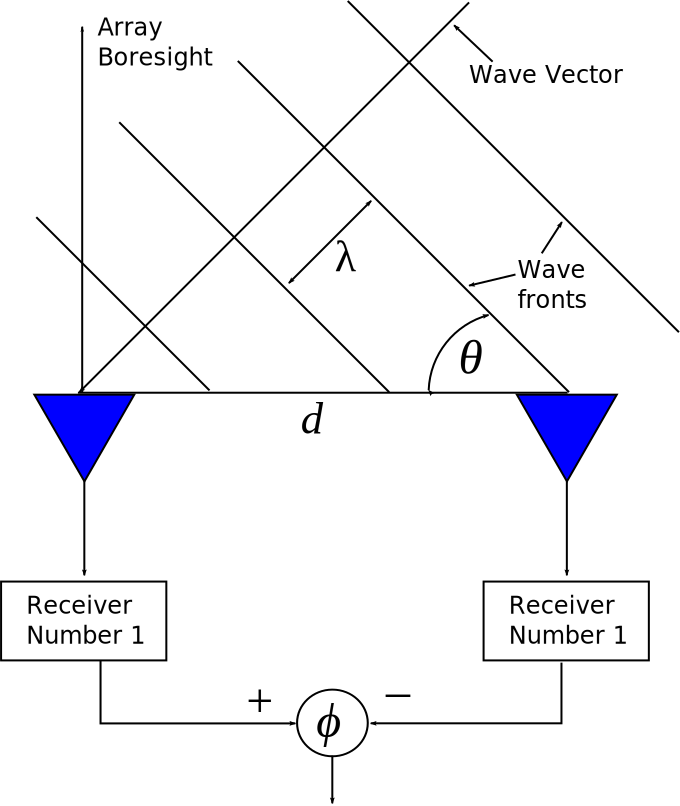
\includegraphics[width=0.4\textwidth]{lit_review/two_element_phase_df_model.pdf}
   \caption{Two-element phase interferometry. Note that as the element spacing (d) is more than half a wavelength there is ambiguity.}
   \label{fig:lit-two-element-phase}
\end{figure}

There are generally three subclasses of phase interferometry systems\cite{jenkins1991smallaperture}:
\begin{description}
  \item [Continuous phase measurement:] A single receiver takes in all of the antenna signals and compares the instantaneous phase of the signals, typically using analogue multipliers. It's fast and relatively simple for two antennas, but becomes complex as the number of elements increases and hence typically has a limited field of view, is susceptible to interference and is not very accurate.
  \item [Phase scanning correlation:] Here, a phase shifter and correlator are used. The phase shifter is varied until the correlator produces a peak output. Again, this is simple for two antennas but becomes complex when multiple phase shifters need to be varied. It is also slow as the phase shift needs to be swept to find the peak correlator output.
  \item [Fourier transform method:] The received signals are digitised and converted to frequency domain, where phase difference measurements are easily taken. As this is a digital technique, spectral processing can be done providing 20 dB to 30 dB of additional sensitivity over the other techniques. Also, working with digital signals in the frequency domain means that phase errors in the signal path can easily be compensated for and adjacent frequency signals can be ignored.
\end{description}
Should the antenna array contain more that two elements, the system either needs to switch between pairs of antennas if it wants to maintain a simple two-input receiver, or it needs a more advanced receiver to sample all antennas simultaneously. The Fourier transform method is the easiest to extend to having more antenna inputs, as the computation is done in the digital domain. Having all antennas processed by the receiver simultaneously allows for a faster system as no switching is required and also provides better performance as it can average multiple inputs at once. However, more inputs requires more computation and algorithmic complexity.

\section{Subspace and Statistical Techniques}
This class of techniques attempts to perform eigen analysis, decomposing the spectral or covariance matrix into eigen subspaces for noise and subspaces for signal. In some sense this equates to a beamforming algorithm which attempts to find an angle resulting in the strongest signal. 
Statistical methods generally involve taking snapshots of the signals received at each sensor, \(\vec{r}(t)\) and then calculating the covariance matrix of the received data\cite{poisel2012electronic}.

The advantage of working with multiple subspaces for each signal is that it allows direction finding to take place when there are multiple overlapping signals arriving at the array. Assume there are \(D\) narrow band signal all with unknown AoA parameter arriving at an \(M\) element array in the presence of uncorrelated noise, the problem space can be reduced from \(M\)-dimensional to \(D\)-dimensional\cite{van2004detection}.

It can be shown that the covariance matrix is diagonal for incoherent sources, non-diagonal and non-singular\footnote{A singular matrix is one which is not invertible, meaning the determinant is 0} for partially coherent sources and non-diagonal and singular if at least one of the sources are coherent\cite{poisel2012electronic}. 

Examples of these techniques include\cite{van2004detection}:
\begin{itemize}
  \item Spectral MuSiC (Multiple Signal Classification) which gets multiple signal snapshots to produce an estimated spectral matrix, \(\hat{\mathbf{S}}_{\mathbf{x}}\) and requires knowing the antenna array manifold vector. It can be applied to arbitrary arrays and performs best when the received signals are uncorrelated. The technique does not work when receiving multiple coherent signals.
  \item Root MuSiC, which is a special form of MuSiC allowing simplified polynomial equations provided linear arrays are used, and requires a lower antenna SNR than Spectral MuSiC.
  \item Least Squares and Total Least Squares ESPRIT (Estimation of Signal Parameter via Rotational Invariance Techniques) which constructs identical subarrays from uniform linear arrays, exploiting shift invariance properties of the array. It can be shown that the signal subspace eigenvectors are linear combinations of the array manifold vector. The RMS error for these techniques can be very close to the Cramer-Rao bound for estimation error\cite{van2004detection}.
\end{itemize}
These subspace techniques typically requires knowledge of the number of unique signals, \(D\), being received as they depend on being able to construct \(D\) subspaces. Seeing as coherent signals degrade performance, they suffer from multipath interference.

\section{Radiometer}
A radiometer is a device which is able to provide a very high accuracy approximation of noise power by averaging a large number of noise samples over a long time period. Due to the high accuracy measurements it can make, it is able to detect small changes in received power. 
It does this by achieving a high sensitivity. Sensitivity is the measure of how weak a signal and instrument is able to detect.

We will define power in terms of a matched load heated to a certain temperature observed over a certain bandwidth.
\begin{equation}
  P = kTB
\end{equation}
where \(k \approxeq \SI{1.38e-23}{\joule\per\kelvin}\), the Boltzmann constant. 

System temperature is a combination of noise powers from atmospheric emissions, the warm earth, the cosmic microwave background, receiver noise figure, losses in the RF chain and others. These noise sources mask the RFI signal which we are trying to locate. While typically an RFI signal below the noise floor would not be an issue, in the case of a radio astronomy reserver that signal will in all likelihood still be a problem because the noise floor of the MeerKAT array is so much lower than the RFI DF instrument. In essence, a signal which will be very loud to the telescope may be difficult for the DF system to even detect. Effort will hence need to go into ensuring that this instrument being designed will be able to see signals below its own noise floor. 

As the noise at an antenna is a combination of a multitude of noise sources, the central limit theorem states that output of the antenna will be approximately a normal (Gaussian) distribution. 

The noise temperature is defined as the noise power per unit bandwidth over the Boltzmann constant:
\begin{equation}
  T_N = \frac{P_v}{k}
\end{equation}

Assuming the power of a noise source remains constant, a single sample of the noise source has an RMS error of approximately \(\sqrt{2}T_{sys}\). However, by integrating the noise power from a certain bandwidth \(\Delta B\) over some integration time \(\tau\) the error can be significantly reduced to
\begin{equation}
  \sigma_{T} = \frac{\sqrt{2}T_{sys}}{\sqrt{2B\tau}} = \frac{T_{sys}}{\sqrt{B \tau}}
\end{equation}
Where \(\sigma_{T}\) is the RMS error in the measurement of the noise temperature, \(T\), and \(T_{sys}\) is the actual system noise temperature. Note that \(2B\tau\) is the number of samples acquired

This process used in a radiometer of acertaining a high accuracy approximation of a received signal by integrating the signal over some observation period can also be used in the context of a direction finding system. For this application, a long observation period may be used to extract a weak signal which is burried in noise so that the weak signal may be processed.

\begin{equation}
  \frac{S}{N} = \frac{S}{N}\sqrt{B\tau}
\end{equation}

Tsys = Tsky + Trx where Tsky is thestuff above and Trx is Johnson noise from electronic components. Tsky can't do anything about. Trx lowered by cooling components. 
The Trx is as a result of the Johnson-Nyquist noise. 

Extension to interferometry:

\(SEFD / (N(N-1))/2 \tau 2B)\)

Sources: \url{https://casper.berkeley.edu/astrobaki/index.php/Radiometer_Equation}
\url{https://casper.berkeley.edu/astrobaki/index.php/Radiometer_Equation_Applied_to_Telescopes}
\url{https://www.cv.nrao.edu/course/astr534/Radiometers.html}


\chapter{System Design}
\label{ch:system-design}

This section will contain an abstracted view of the system, with blocks for antanna array, RF front end, digitisers, first stage DSP on ROACH, 2nd stage DSP on PC with ethernet link.

A brief explanation of the design considerations for each stage of the system. Stating that each block will be designed and expanded on in the following chapters.

\chapter{Antenna Array and RF Front End}
\label{ch:rf-front-end}
\setsvg{svgpath=./img/rf-front-end/}
\graphicspath{{./img/rf-front-end/}}

This chapter details the design and characterisation of the antennas and RF front end; the first sub-system in the direction finder. The RF front end consists of low noise amplifiers (LNA), lower pass filters, and cabling. As discussed in the previous chapters, the aspects of the array which needs to be optimised for are:
\begin{itemize}
  \item Minimize the phase difference the RF path for each antenna. The DF algorithm is based on phase/time difference measurements and hence path mismatches will result in errors. Some phase difference can be calibrated out but the calibration routine will be most robust when the initial error is low.
  \item The spacing of the elements in the circular array needs to trade off between too large an element spacing and too small a spacing. Too large will result in phase ambiguity, to small will result in coupling between the elements as well as difficulty in measure time difference. The compromise is to make the array as large as possible before phase ambiguity becomes a problem.
\end{itemize}

The ADCs which were available for use in this project influenced the antenna and operating frequency band choice. They're explored more in Chapter 5 but will be briefly noted here as justification for the decisions taken here. The ADCs were two dual-input cards which sample two inputs in phase. They were clocked up to \SI{800}{\mega\hertz}. This implies 4 simultaneous inputs with a Nyquist frequency of \SI{400}{\mega\hertz}.\\

The Chapter will first discuss the design and construction of the antenna array, then move on to the RF front end. Finally, characterisation of the amplitude and phase performance of the RF front end will then be done. 


\section{Antenna Array}

As shown in the simulations, it's preferable to use an odd number of elements in the circular array as the phase ambiguity is reduced when there are no lines of symmetry. However, there is a constraint in the hardware that's being used for this project: there are a total of four simultaneous ADC inputs. Rather than going down to three elements, all four inputs will be used but the circular array will be deformed in order to remove the lines of symmetry. The amount of deformation will be trade off between deviating too far from a circle and hence having performance that is not the same in all directions, or being too close to a circle and hence suffering from ambiguity. This project does not go into depth on array deformation strategies; the array design is proof of concept and the deformation we can do is limited by the mounting hardware. A few array geometries were tried and the one that performed best in ambiguity simulation.

\begin{figure}
  \centering
  \includegraphics[width=0.4\textwidth]{antenna-array-on-roof}
  \includegraphics[width=0.59\textwidth]{antenna-s11}
  \caption{Array of four FD-250 folded dipoles being measured and the result of the S11 measurements showing acceptable performance between \SI{200}{\mega\hertz} and \SI{300}{\mega\hertz}.}
  \label{fig:rf-front-end:antenna-array-s11}
\end{figure}

Four FD250 folded dipole antennas with a center frequency of \SI{250}{\mega\hertz} were sourced. This centre frequency was picked as it's around the middle of the \SI{400}{\mega\hertz} ADC usable bandwidth. The antennas were mounted in a deformed circle. Measurements were taken and acceptable S11 performance in the band of interest was observed; see \Cref{fig:rf-front-end:antenna-array-s11}.

In order to be able model the array in simulations and field trials, it was necessary to get coordinates for each element. A Python program was written which takes is input measurements of all of the baselines and does a least square errors calculation to estimate the coordinates of each element. A top down view of the real array as well as a plot of the elements produced by the script is show in \Cref{fig:rf-front-end:array-coordinates}.
Thoughts on what could go here:
- show multi-colour vis vs df error graph
- show individual fixed source plots
- show fixed freq 4 vs 4 deformed plots
- link to appendix for individually samples plots.

%TODO: put the following back
\begin{figure}
  \includegraphics[width=0.4\textwidth]{array-top-view}
  \includegraphics[width=0.59\textwidth]{array-coordinates}
  \caption{Top view with coordinates}
  \label{fig:rf-front-end:array-coordinates}
\end{figure}

\begin{figure}
  \centering
  \begin{subfigure}{\textwidth}
    \centering
    \includegraphics[width=0.90\textwidth, clip=true, trim = 0 14 50 0]{4}
    % left, bottom, right, top
  \end{subfigure}
  \begin{subfigure}{\textwidth}
    \centering
    \includegraphics[width=0.90\textwidth, clip=true, trim = 0 14 50 0]{4-deformed}
  \end{subfigure}
  \caption{Ambiguity plots for various antenna array sizes with reference signal arriving at \SI{0}{\degree} showing improved ambiguity after array deformation.}
\end{figure}

\begin{figure}
  \centering
  \includegraphics[width=0.7\textwidth, clip=true, trim = 0 0 60 0]{4-element-circular-ambiguity-vs-phi}\\2em
  \includegraphics[width=0.7\textwidth, clip = true, trim = 0 0 0 0]{4-element-deformed-ambiguity-vs-phi}
  % left, bottom, right, top
  \caption{Some caption here}
\end{figure}

RMS phase error vs RMS angular error. MOVE THIS TO FRONT-END SECTION.
\begin{figure}
  \centering
  \includegraphics[width=0.9\textwidth]{visibility-error-vs-df-error}
  \caption{This is a graphic showing some stuff}
\end{figure}

Again, simulation:
SNR vs number of correct correlation peaks.
Table: 
For an SNR: Do 1000 different cross correlations.RMS error in number of samples.
Do SNR: 10, 5, 2, 1, 0.5, 0.2, 0.1

\section{RF Front End}

\begin{figure}
  \centering
  \begin{subfigure}{\textwidth}
    \centering
    \includesvg[width=\textwidth]{fr-front-end-circuit-sch}
    \caption{Schematic of the RF front end circuitry.}
  \end{subfigure}\\[1em]
  \begin{subfigure}{\textwidth}
    \centering
    \includegraphics[width=0.6\textwidth]{rf-front-end-charging}
    \caption{Board containing amplifiers and filters in the corner, batteries velcroed down on the sides, and regulators and connectors on the veroboard in the middle.}
  \end{subfigure}
  \begin{subfigure}{\textwidth}
    \centering
    \includegraphics[width=0.6\textwidth]{lpf-in-holder}
    \caption{Close up of a low pass filter connected to an amplifier, held down to make it more rugged in the field.}
  \end{subfigure}
  \caption{RF front end design and construction.}
  \label{fig:rf-front-end:circuit-board}
\end{figure}

The RF front end is responsible for filtering and amplifying the signals, being the bridge between the antennas and the ADC. As discussed in Chapter 3, it is necessary for an interferometry system to have its RF front end components phase and amplitude response approximately matched.
The ADCs have \SI{400}{\mega\hertz} of usable bandwidth and the antennas have a centre frequency of \SI{250}{\mega\hertz}. Hence, the filtering should cut off before \SI{400}{\mega\hertz} and the amplification should occur around \SI{250}{\mega\hertz}. 

Suitable parts were purchased. The LNAs which are used are the ZLF-500HLN from MiniCircuits. This part operates from \SI{10}{\mega\hertz} to \SI{500}{\mega\hertz} which is ideal for the application. The gain is approximately 21 dB across this band according to the datasheet, drawing up to \SI{110}{\milli\ampere}.  The low pass filters (LPF) which were purchased are VLF-225+ parts from MiniCircuits having a \SI{3}{\decibel} point at \SI{350}{\mega\hertz}, which defines the usable bandwidth of the RF front end.

The RF front end needs to be able to be taken out into the field and used while running on batteries.
Two ZIPPY Compact \SI{1000}{\milli\ampere\hour} 3S 25C battery packs and 4 LM7815 regulators were acquired. 
Each amplifier has its own regulator to try to reduce any electrical coupling between the regulators through their power rails.
The battery packs output \SI{12.5}{\volt} when fully charged meaning a combined input to the \SI{15}{\volt} regulators of \SI{25}{\volt}. Hence the regulators are dropping \SI{10}{\volt} at \SI{100}{\milli\ampere} or \SI{1}{\watt}.
The LM7815s can handle this dissipation provided a heat sink is connected, which was done.
This power distribution circuitry was put onto veroboard.

All of the amplifiers and filters and the power distribution circuit were mounted to a wooden board.
Care was taken to make sure that the low pass filters were securely and firmly attached to the board as there is a risk that the SMA connector would snap off if they they were bumped. 
The circuit diagram for this board and the resulting hardware implementation for this RF front end are are shown in \Cref{fig:rf-front-end:circuit-board}.

Finally, the cables need to be carefully matched as well. Provided the cables are of the same type, their velocity factors will be equal and it is hence only necessary to ensure that they are of the same length. The LPFs and LNAs however may have phase mismatches due to manufacturing tolerances. 

In order to check whether the LNAs provide the expected gain and to check whether the phase matching of the RF front end is good, the whole subsystem of cables, amplifiers and filters were connected to a network analyser and S21 measurements taken. The results are shown in \Cref{fig:rf-front-end:vna-measurements}. It can be seen that the amplitude drops off rapidly at around \SI{400}{\mega\hertz} providing necessary anti aliasing. At \SI{350}{\mega\hertz} the difference between the in band signal and the aliased signal is almost \SI{-30}{\decibel} which is sufficient isolation to consider the system usable up to \SI{350}{\mega\hertz}. The phase matching is good, within a degree or two over the whole band of operation.

\begin{figure}
  \centering
  \begin{subfigure}{\textwidth}
    \centering
    \includegraphics[width=0.6\textwidth]{zfl500-10-3000}
    \caption{Gain from 0 to \SI{3}{\giga\hertz} in dB. Antialisaing is sufficient. The iADC is only receptive to signals up to \SI{3}{\giga\hertz} so it's only necessary to look at filtering up to there.}
  \end{subfigure}\\[1em]
  \begin{subfigure}{\textwidth}
    \centering
    \includegraphics[width=0.6\textwidth]{zfl500-10_500-mag-db}
    %\caption{Gain from 0 to \SI{500}{\mega\hertz} in dB. Useable seems to be up to \SI{350}{\mega\hertz}}
    \caption{VNA measurements of S21 of RF chains showing antialising properties}
  \end{subfigure}
  \begin{subfigure}{\textwidth}
    \centering
    \includegraphics[width=0.6\textwidth]{zfl500-10-500-phase}
    \caption{Phase from 0 to \SI{500}{\mega\hertz} showing very good phase matching over operating frequency range below \SI{350}{\mega\hertz}}
  \end{subfigure}
  \caption{S21 measurements of RF front end subsystem.}
  \label{fig:rf-front-end:vna-measurements}
\end{figure}


\section{Summary}
This Chapter has detailed the design, construction and measurement of the antenna array and RF front end subsystem. It's shown how a 4 element array can be deformed from a square to produce ambiguity performance that's not far off of what's achieved by a 5 element array. Code was written to be able to introduce a coordinate system to elements from baseline distance measurements. 

The RF front end was built to provide some amplification in the band of interest and attenuation of out-of-band aliased signals. Mounting the circuitry on a board and making it battery powered will allow it to be taken into the field easily.

Measurements of the performance of the RF front end show it should work as expected.

\chapter{FPGA Firmware}
\label{ch:firmware-design}
\setsvg{svgpath=./img/firmware/}
\graphicspath{{./img/firmware/}}

This Chapter details the design, implementation and testing of the FPGA firmware. Testing involves both simulating using data path as well putting the firmware on the physical FPGA, sending input RF signals to it and analysing the output of the FPGA's DSP.

\section{Hardware Specifications}

\begin{figure}
  \centering
  \includegraphics[width=\textwidth]{roach-photo}
  \caption{Photo of the ROACH board and ADCs. Bottom: Two Atmel AT84AD001B dual ADC cards with SMA connectors going in to them and connected via Z-DOK to the ROACH board. Bottom right: ADC clock synthesiser feeding into power splitter which in turn clocks each ADC board in phase. Top: main ROACH board. The Virtex-5 is under the blue fan. To its left is the ROACH's DRAM module. To the right of the fan is the PowerPC with its DRAM module.}
  \label{fig:firmware:roach-photo}
\end{figure}

As discussed in the user requirements, the FPGA processing board that should be use is the same which is used by the SKA: the Reconfigurable Open Architecture Computing Hardware (ROACH)\footnote{\url{https://casper.berkeley.edu/wiki/ROACH}} board. This board has a Xilinx Virtex-5 FPGA on it, with connectors for Z-DOK+ cards which will be used for ADCs and a DDR2 DRAM connector for high volume\footnote{Compared to the Virtex-5's on-chip storage} data storage. There is a PowerPC subsystem on the ROACH running Linux which provides a 1 Gbps Ethernet interface for programming and data readout from the memory of the FPGA. The PowerPC runs a daemon called tcpborphserver which speaks the KATCP protocol used to interact with the ROACH. There are other blocks on the ROACH board as well, but the ones listed here will be the ones utilised in this project.

There are various ADC cards compatible with the ROACH. The ones which were made available for this project are iADC cards. Each card has an Atmel/e2V AT84AD001B 8-bit dual ADC chip on it. It's designed for I/Q sampling but can be configured to sample both channels in phase; exactly what's needed here. The clock speed can be up to \SI{1}{\giga\hertz} and must be externally supplied. The ADC feeds the clock signal through to the FPGA along with the sampled data with a demux factor of 4:1 meaning that for every 4 ADC clock cycles and 4 samples, the FPGA gets one clock cycle with all 4 samples on the ADC data bus. This implies that the FPGA will run at exactly a quarter of the speed the ADC runs at, and needs to be able to handle 4 samples per channel times 4 channels = 16 samples every clock cycle.

The clock source is a Valon 5007 dual synthesiser which is USB programmable from \SI{137}{\mega\hertz} to \SI{4400}{\mega\hertz}. Both ADCs need to be clocked exactly in phase so the Valon is fed into a Mini-Circuits ZESC2-11+ power splitter which has a low phase imbalance.

The ROACH board with connected ADCs is shown in \Cref{fig:firmware:roach-photo}. All of the components are in a metal case for RF shielding, although the cover has been removed for the photo.


\section{Firmware Development Toolchain}
There are a few components necessary to get development for the ROACH working. They're briefly listed here and detailed more in \Cref{appendix:roach-development}.\\

Xilinx ISE 14.7 is needed for synthesising (compiling) HDL files to FPGA bitfiles. This proprietary tools is maintained by Xilinx and made available through the SKA. As well as this key task of compilation it also has peripheral tools for debugging and optimisation which proved useful for getting the design to meet timing. More info in \Cref{appendix:roach-development}. Although it also works on Debian/Ubuntu systems, ISE is most stable and only officially supported for RHEL. As such as CentOS system was used for FPGA development work as it's mostly the same as RHEL at the binary interface level.\\

Matlab R2012B with Simulink was installed, along  with the mlib-devel plugin. The majority of the design work for ROACH done in this project is done at the block diagram level in Simulink. There is a plugin called mlib-devel which defines the Simulink interface for the Xilinx cores, as well as containing HDL code for ROACH specific hardware such as ADC cards, DRAM interface and PowerPC control bus. This naturally includes the net definitions for the components on the ROACH board.

The mlib-devel plugin was originally created by CASPER, now contributed to extensively by the SKA. It contains a multitude of highly useful DSP blocks which are built on top of the Xilinx cores which can be wired up in Simulink. These include range from relatively simple blocks like edge detectors to very complex ones like real-time FFT blocks and polyphase filterbank blocks. Additionally, blocks for interfacing with hardware like ADCs, memory, shared registered and generic IO are included. It was necessary for this project to update some blocks during this project, hence a clone of this mlib-devel repo was created\footnote{\url{https://github.com/jgowans/mlib_devel}}.


\section{Design}
There are a number of subsystems developed for the FPGA which will be discussed here. Most of these subsystems required extensive development, testing and tweaking. The full design is shown in \Cref{fig:firmware:full-design}. It may be difficult to see all of the detail of the design, but the purpose of the figure is to give an indication of the structure, layout and data flow in the FPGA. The following subsections discuss the purpose of the key blocks in the design. A more detailed look at the composition and structure of the some of the blocks can be found in \Cref{appendix:roach-development}. That Appendix also discusses the challenges that were encountered during the FPGA design, and the optimisations that were done to get it working.

\afterpage{%
  \clearpage% 
  \begin{landscape}
    \thispagestyle{empty}
    \begin{figure}
      \vspace{-4em}
      \centering
      \makebox[\textwidth][c] {
        \includegraphics[width=1.22\paperwidth,center]{full-design-a4-no-sim-out.pdf}%
      }%
      \caption{Full FPGA design containing frequency and time DSP paths and control logic.}
      \label{fig:firmware:full-design}
    \end{figure}
  \end{landscape}
}

\subsection{ADCs}
The yellow blocks on the left represent the two dual ADCs. These \(2 \times 2\) channels will be referred to as channel 0, 1, 2 and 3. Each ADC has \(2 \times 4 = 8\) 8-bit buses for the signed integer samples that are clocked in every clock cycle. As mentioned earlier the FPGA runs at a quarter of the ADC clock cycle hence the ADC presents 4 samples per clock cycle.  Also included are logic lines that indicate clipping. For simulation purposes, normal Simulink signal source blocks can be connected to the ADC, allowing the construction of arbitrarily complex input signals. The example shows a simple chirp connected. The output from the ADCs fans out to two distinct signals paths: a frequency domain path and a time domain path. These are now explored.

\subsection{Frequency domain signal path}
The frequency domain path starts with an FFT block, the first big green one,  which performs real time FFTs on the data from the ADCs. Although it's one block it does four distinct Fourier transforms under the hood, one for each of the ADC channels. It's an 11 stage FFT meaning that it does \(2^{11} = 2048\) points. It has an optimisation for real-valued signals in that it only output the positive half of the frequency spectrum to save bandwidth. The FFT has been configured to do full bit growth, meaning that every stage another bit of data is added to the bus size. This means that weak signals will be preserved as no bits are thrown away. This is at the expense of significant data growth: each channel outputs two 36-bit complex numbers every clock cycle.

FFT output is fed into the second big green block, the Cross Multiplier. This does \({4 \choose 2} = 6\) cross multiplications, one for each baseline, as well as one additional for the autocorrelation of channel 0 to serve as a spectrum analyser. These are referred to as 0x0, 0x1, 0x2, 0x3, 1x2, 1x3 and 2x3. The cross multiplication involves breaking the signal up into its real and imaginary component, taking the complex conjugate of one of the signals by inverting the sign of its complex component and then doing complex multiplication. For each pair of signals signals \(A\) and \(B\) where \(A = (a + ib)\) and \(B = (c + id)\) the FPGA will do \(C = A\overline{B} = (ac + bd) + (bc - ad)i\). The cross multiplier does not throw any bits away meaning that the signals go from a \(2 \times 36 = 72\) bit complex numbers to 148 bits per channel.

The cross correlation signals then go to the white Accumulators block. As discussed in Chapter 3, the cross correlations will be accumulated (aka: integrated) a number of times in order to allow weak signals to stand out of the noise. The accumulation length is runtime programmable via a control register which will be discussed more later. The accumulator works by using FPGA BRAM to produce a delay, and a DSP48E to add the new signal to the current one. The length of the BRAM is the number of points in the FFT spectrum, 2048. The accumulators allow signal growth from 74 bits per complex number to 96 bits. This implies a minimum of \(\approx 4\) million accumulations when the signals are full scale, although typically this can be orders of magnitude more as the system does not run with full scale input; it's too dangerous the keep the ADCs at max power.

Each accumulated correlation value is wired to its own BRAM snapshot block, the array of small green blocks on the right. Once sufficient accumulations have been run, the snapshot blocks are triggered to take a snapshot of the correlation spectrums. The snapshots then record the full accumulated correlation spectrum of a channel, now 128 bits wide per frequency channel per correlation pair, to shared BRAM memory. This memory can then be read out from the FPGA via the PowerPC over Ethernet.

\subsection{Time domain signal path}
This path is comparatively simpler than the frequency domain path, seeing as the correlations are not being done on the FPGA, and seeing as accumulation is not applicable for time domain DF. 

There are two main blocks for the time domain path, which are at the bottom of the FPGA design. First is the impulse detector. This takes in the raw ADC data from channel 0 and runs a rolling sum filter which provides the sum of the last \(N\) samples where \(N\) is some runtime programmable number, typically between 10 and 1000 samples. If the rolling sum goes above a runtime programmable threshold the impulse detector considers an impulse to be present. It then records the raw time domain data of all 4 channels for as long as the impulse is present, plus some additional buffer at the start and end of the pulse.  The snapshot is stored by the green block at the bottom, the off-chip DRAM module. The starting buffer is attained by feeding a delayed version of the raw signal to the DRAM interface. The DRAM module was chosen as it can store a large amount of data, allowing multiple milliseconds of raw data to be stored if desired. Typically only a few microseconds of data is necessary to store an impulsive signal. As well as triggering the snapshot, the impulse detector will also store the length of the impulse which it detected so that the computer knows much data to read out from the DRAM module when it wants the data. The DRAM data is also accessible through the PowerPC over Ethernet.

\subsection{Control and Monitoring}
The FPGAs runtime configuration and status can be interacted with via shared memory accessible in the address space of the PowerPC. This memory manifests as as words of data registers on the FPGA. Slices of these registers are wired to different parts of the FPGA logic to dynamically change it in the case of writable memory, or to get status info in the case of readable memory. The registers are the yellow blocks dotted around the design. Following are a few control and monitoring functions. The description of what they do also indicates more about how the design works.
\begin{itemize}
  \item Integers for accumulation length, impulse detector rolling filter length and impulse detector setpoint. These are all separate 32 bit registers for runtime configuration of these values.
  \item Impulse detector arm. The impulse detector will only write a snapshot to DRAM if its threshold is breached while the arm latch is high. The latch is cleared when a snapshot is detected, and can be set again by the computer once the snapshot has been read out. The reason for this is to prevent the race condition where a new snapshot could partially overwrite an earlier one which is busy being read out by the computer.
  \item Snapshot trigger gate. Similar to the reasoning behind the impulse detector arming, this gate to all of the snapshot trigger blocks exists to prevent a new accumulated spectrum from being written on top of one that is being read out. The computer will gate the trigger while it's busy reading the snapshot blocks, and clear the gate once the readout is complete.
  \item Rolling sum level. This is the current value of the rolling sum filter. By watching the value of the filter for some time, an informed decision can be made about where to put the setpoint for the impulse detector. Typically this would be a few standard deviations above the mean. Setting its value is a trade off between false positives and false negatives.
  \item Impulse length. The impulse detector records how long the impulse goes on for. The computer can poll this value to see how much data needs to be read from DRAM. By reading only the minimum data, the readout is faster and the time domain cross correlation is more accurate.
  \item Overflow status latch and reset. The various parts of the system which can overflow feed latched version of their overflow status lines into a register. Then, whenever a snapshot is read out the overflow register is examined as well so see if the data should be treated as valid or not. There are multiple bits so it can be seen which part of the system overflowed and configuration can be adjusted to remediate this overflow. For ADC overflow this would be adding analogue attenuators. For accumulation overflow this would be reducing the accumulation length. For FFT overflow this would be changing the shift schedule. As well as going a register to be read out by the computer, this overflow latch is also fed to GPIO register which drives an LED mounted on the ROACH case so that should any overflow happen it will immediately light the LED to inform the operator. The computer can acknowledge the occurrence of overflow by pulsing a reset line which will clear the latch.
  \item Manual sync pulse. Data is streamed into the FFT block and frequency channels come out in order which eventually need to be stored in snapshot memory, lowest numbered channel at the start and highest channel at the end. As such, something needs to keep track of which channel is the first one. The sync pulse achieves this by resetting the FFT, and the FFT will then output the sync pulse at the same clock cycle as channel 0. This sync pulse is then propagated through the multipliers and in to the accumulators, which ensures that the start of an accumulation is in phase with the start of a spectrum. This sync line is pulsed by the computer when it connects to initialize the data path.
  \item Accumulation counter. Every time an accumulation is completed and a new one started, this counter increments. The computer can use this to know when it's time to read out a new spectrum and also to ensure it's keeping up and reading out all snapshots.
  \item FFT shift schedule. Sets which phases the FFT should shift data down by 1 bit and when it should allow bit growth. It ended up not being needed as it was possible to fit a full bit growth FFT on to the design. However, should a longer FFT or other additional logic be needed in future, it will be necessary to shrink the width of the data path and then use a shifting FFT.
\end{itemize}

\section{Simulation}
\begin{figure}
  \begin{subfigure}{\textwidth}
    \centering
    \includegraphics[width=0.8\textwidth]{impulse}
    \caption{Periodic \SI{1}{\micro\second} impulse at half of the power of the noise}
  \end{subfigure}
  \begin{subfigure}{\textwidth}
    \centering
    \includegraphics[width=0.8\textwidth]{noise}
    \caption{Additive Gaussian white noise}
  \end{subfigure}
  \begin{subfigure}{\textwidth}
    \centering
    \includegraphics[width=0.8\textwidth]{impulse-plus-noise}
    \caption{Sum of impulse and noise. Impulse is not distinguishable by eye.}
  \end{subfigure}
  \begin{subfigure}{\textwidth}
    \centering
    \includegraphics[width=0.8\textwidth]{filter}
    \caption{Output of moving sum filter. Additional noise power now clearly visible}
  \end{subfigure}
  \caption{Simulink simulation of how filter can detect impulse even below noise floor.}
  \label{fig:firmware:impulse-detection-simulation}
\end{figure}
As the design is created in Simulink, the extensive simulation capabilities it provides can be used to validate that the design should behave as intended. Simulation was used throughout the development process, for both the time and frequency domain signal path. For example, for the frequency domain path a repeating correlated chirp signal with a defined start and end frequency would be injected in the input, and the snapshot blocks would be examined to ensure that there was a flat power spectrum between those frequencies. For the time domain path, short impulses in the presence of noise were simulated, and the output of the rolling average filter monitored to ensure that it correctly detected a rise in power. An example of this is shown in \Cref{fig:firmware:impulse-detection-simulation}. This example has the extreme case where the impulse is actually smaller than the additive noise, yet the filter is able to detect it and could trigger a capture of it.

\section{Design compilation}
Over the course of this research, the design developed from being a simple two-antenna time domain data collector to the full four-antenna time and frequency domain DSP subsystem described here. The full design is very large, consuming more than 95\% of the available logic on the FPGA. Numerous optimisation were necessary to get it to fit which are detailed more in \Cref{appendix:roach-development}.

Part of the compilation process involves defining the clock speed at which the FPGA should operate. The Xilinx tools then move logic around to ensure that all signals can propagate and be valid in the necessary time. Hence faster speeds are more difficult to compile as it's more likely a path will not meet timing. The timing value that proved reliable for this design was \SI{200}{\mega\hertz}. This implies an ADC clock speed of \SI{800}{\mega\hertz}. The ADCs have a maximum clock speed of \SI{1000}{\mega\hertz} so this speed is fine for them. 

The ADC's \SI{800}{\mega\hertz} sample rate implies a Nyquist frequency of \SI{400}{\mega\hertz} which explains why \SI{400}{\mega\hertz} has been used extensively in the previous sections for DF algorithm simulations and antenna design.

\section{Lab Tests}
In order to validate that the FPGA subsystem was working as expected, a hardware setup was created in the lab to emulate the sort of signals which the DF system would see in the field. The setup contained signal sources for both strong impulsive signals, as well as weak narrow band tone signals. The impulses and tones were split and fed to all ADCs. As well as getting the correlated signals, uncorrelated noise was added, allowing more accurate tests ensuring that the correlation and accumulation part of the DSP path could extract weak signals from noise. The physical setup in the lab is shown in \Cref{fig:firmware:lab-setup-photo} with a diagram of the configuration in \Cref{fig:firmware-lab-setup-diagram}. 

This hardware rig was used during development in conjunction with the Simulink simulations to ensure that the running design was operating as intended. 

For the time domain path the tests involved arming the time domain capture, then manually triggering a one-shot impulse. The system successfully detected the impulse and captured it on all four channels, was well as its length with some start and stop buffer to DRAM. This signal could then be read out.

The frequency domain path tests involved producing a tone at a certain frequency and ensuring that accurate phase difference as seen by each input was seen after accumulation. The expected phase was set by feeding different cable lengths from the splitter to the ADCs. Two situations were tested, one where all cables were of equal lengths hence expecting to see \SI{0}{\degree} phase shift between all baselines. The other test was where one cable was longer than the rest, hence expecting some of the baselines to see a phase shift while others to be in phase. The expected phase shift was checked by measuring the cables on a network analyser. These tests were done at different SNR levels to quantify not only that the observed phase shift was present but also how performance changed with SNR level and with accumulation length. Results for SNR levels of 0.1, 0.01 and 0.001 are shown in Figure 5.6. Note that these SNR levels are for the noise power in just the channel of the signal, not total noise power. Total noise power is order of magnitudes higher as the white noise has power across the whole spectrum. These results show that the system is behaving as expected in two key ways. First, in general, error diminishes as more samples are accumulated. Second, the higher the SNR the faster the lower the faster the error drops off. Based on these results we can say that the system is able to operate all the way down to SNR levels of 0.01 provided integration time can span hundreds of thousands of samples, or a few seconds.

\begin{figure}
  \centering
  \includegraphics[width=\textwidth]{lab-setup-photo-labeled-resized}
  \caption{Equipment setup in the lab. Top to bottom: ROACH; four noise sources; RF splitters, combiners and attenuators; RF board with amplifiers and filters; impulse generator; trigger and gate for impulse generator; signal generator for narrow band signals}
  \label{fig:firmware:lab-setup-photo}
\end{figure}
\begin{figure}
  \centering
  \includegraphics[height=\textheight]{lab-setup-diagram}
  \caption{Diagram showing how the various components in \Cref{fig:firmware:lab-setup-photo} are connected together.}
  \label{fig:firmware-lab-setup-diagram}
\end{figure}

\afterpage{%
\thispagestyle{empty}
\begin{figure}
  \vspace{-4em}
  \begin{subfigure}{\textwidth}
    \centering
    \includegraphics[width=0.7\textwidth]{integration-vs-error-0x1-2}
  \end{subfigure}
  \begin{subfigure}{\textwidth}
    \centering
    \includegraphics[width=0.7\textwidth]{integration-vs-error-0x01-2}
  \end{subfigure}
  \begin{subfigure}{\textwidth}
    \centering
    \includegraphics[width=0.65\textwidth]{integration-vs-error-0x001-2}
  \end{subfigure}
  \caption{Plots for integration length vs output error tests in SNRs of 0.1, 0.01 and 0.001. Each line on the graph is an iteration of the test.}
  \label{fig:firmware:phase-error-measurement-plots}
\end{figure}
}


\section{Summary}
This Chapter has first discussed the DSP signal paths in the FPGA design, including the frequency domain cross correlation and accumulation path, and the time domain rolling sum filter and impulse detection paths. It also discussed the control and monitoring blocked used to interface with a computer. Next, it was shown how the design has been tested and verified, using both Simulink simulations and a hardware setup in the lab. The hardware setup has RF sources for impulses, tones, and uncorrelated noise. The performance of the system was as expected, being able to detect and capture impulses, as well as measure the phase of tones which were well below the noise floor.

\chapter{Software}
\label{ch:software-design}
\setsvg{svgpath=./img/software/}
\graphicspath{{./img/software/}}
Software was written in Python to run on a computer which is connected to the ROACH via Ethernet. The software has two broad functions: to interact with and provide an abstraction to the FPGA, and to perform angle of arrival estimation based both on the received signals and on the antenna model. This Chapter looks at the structure of the software package and some results indicating it is working as expected.

\section{Code Structure}
\begin{figure}
  \centering
  \makebox[\textwidth][c] { 
    \includegraphics[width=1.1\textwidth, clip=true, trim = 80 365 80 80]{backend-arch}
    % left, bottom, right, top
  }
  \caption{UML class diagram of software structure in \lstinline{DirectionFinder-backend}.}
  \label{fig:software:df-backend-uml}
\end{figure}
The code had to be designed in accordance with good object-orientated methodologies in order to provide a useful, well defined and easily extendible interface to the various software components which need to interface with one another and with the correlator. As such, there was significant emphasis encapsulating logic into classes which mirrored the physical structure of the correlator and the antenna array with regard to modularising key components and writing reusable code.

The main package containing the array modeling, the ROACH interface and the AoA estimation is \lstinline{DirectionFinder-backend}\footnote{\url{https://github.com/jgowans/directionFinder_backend}}. The structure of the classes in this package is shown as a UML diagram in \Cref{fig:software:df-backend-uml}. The root class, \lstinline{DirectionFinder} is composed of an \lstinline{AntennaArray} and a \lstinline{Correlator}. 

The \lstinline{AntennaArray} is initialised from an array geometry file that has been produced by the element coordinate calculator discussed in Chapter 3. It is able to return expected baseline phase shifts or time delays for all antenna pairs at any angle. The returned values are used to get the theoretical array response for a given angle at a specific frequency. Due to the modular structure of the \lstinline{AntennArray} class, it can be used to simulate and provide information about an antenna array with any number of elements in any configuration. This is an example of the general purpose nature of the application which is being developed here.

The \lstinline{Correlator} provides an interface to processed data from the FPGA. It is able to fetch both frequency domain cross correlations from the snapshot blocks as well as time domain snapshots which it gets by reading raw time domain data and doing in-memory time domain cross correlations. The \lstinline{Correlator} also contain a \lstinline{ControlRegister} which abstracts the raw bit or word read/writes necessary to interact with the status and configuration registers. Once again the software has been designed with generality in mind: any number of baselines can be read out, having spectrums with any number of points for arbitrary start/stop frequencies. These are initialisation configuration parameters of the classes providing the abstractions.\\

The software application is launched by a Python executable which takes command line arguments that define the IP of the ROACH, the path to the configuration file for the ROACH, the frequency domain start/stop frequencies, the frequency or frequency range which should be monitored for direction-finding, impulse setpoint, accumulation length, and a comment string to label the observation which is being made. Once running, the software will monitor for impulses and it will continuously DF the narrow band signal. The raw baseline measurements as well as the calculated AoA are both printed to the screen and are written to a log file in a format which can easily be post-processed for plotting. Warnings such as overflow are printed to the screen.\\

The following sections explain how the software goes about ascertaining angle of arrival for time and frequency domain signals.

\section{Frequency Domain Direction Finding}
The frequency domain DF algorithm assumes that the signal of interest may well be below the noise floor. As such, no detection is done; the direction finding is continuous. 

When the application starts up, it reads in the array configuration file and constructs an \lstinline{AntennaArray} object from it. It then samples the antenna array manifold vector at \SI{0.36}{\degree} intervals, corresponding to 1000 baseline phase shift vectors. These are stored in a hash in memory. 

Next, the ROACH is initialised by writing to the accumulation length (\lstinline{acc_len}) register and pulsing the \lstinline{sync} line. The accumulation length value is set based on user input, typically it will be around 1 second. Next, it constructs instances of a \lstinline{Snapshot} class, one for each baseline cross correlation BRAM snapshot on the FGPA. These snapshot blocks are all armed, and once armed the snapshot trigger ungated. The system sits in a tight loop watching the accumulation counter. When the accumulation counter ticks, the snapshot trigger is gated and all snapshot values read out. Calibration factors (discussed more later) are then applied to the signals. The strongest signal in the frequency interval of interest is found, and the phase shifts as seen by each baseline correlation are fetched and stored in a map of baseline name (eg: ``1x3'')  to phase shift. Finally, the \lstinline{DirectionFinder} iterates through all 1000 simulated angles, comparing the simulated baseline phase shifts to the observed baseline phase shifts and selects the angle whose simulated values most closely match the observed values. In pseudo code:

\begin{lstlisting}
AntennaArray antenna_array = new AntennaArray(config_file)
Correlator correlator = new Correlator(...)

while True:
  Correlation correlation = correlator.get_correlation()
  Float frequency = correlation.strongest_signal_in_range(f_start, f_stop)
  Map<Baseline, Float> observation = correlation.baseline_phase_shifts_at(frequency)

  Float best_angle = 0;
  Float lowest_difference = INT_MAX;

  for angle in antenna_array.sampled_angles
    Float difference = antenna_array.manifold_at(frequency, angle).compare(observation)
    if difference < lowest_difference:
      best_angle = angle;
      lowest_difference = difference
  write_result(best_angle)
\end{lstlisting}

The \lstinline{compare} method computes the difference between vectors by the RMS of the difference of their terms. When the difference, \(d\) is computed for two vectors \(\vec{a}\) and \(\vec{b}\) with \(k\) terms, it uses arctan to account for the fact phase wraps around \(2\pi\), as follows:

\begin{equation}
  d = \left[ \sum_{i=0}^{k}\abs{\atantwo(\sin(\vec{a}_i - \vec{b}_i), \cos(\vec{a}_i - \vec{b}_i))}^2 \right]^{1/2}
\end{equation}


\section{Time Domain Direction Finding}

As mentioned in Chapter 3, the algorithm behind time domain DF is remarkably similar to frequency domain DF. The main difference is that the comparison method uses baseline time delays rather than phase shifts. 

One important difference is that where the frequency domain cross-correlations are calculated using DSP on the FPGA, the time domain cross-correlations need to be calculated on the computer. This is not a hard requirement, but the implementation of the FPGA design did not cater for time domain cross-correlations which can be a lot trickier to do in hardware since the length of the pulse is dynamic.

The time domain cross-correlation is implemented, as defined, by multiplying each point of one antenna's signal \(\vec{a}\) by the corresponding points of a shifted version of another antenna's signal \(\vec{b}\) for some shift \(k\), producing the correlation \(c_{ab}(k)\):
\begin{equation} \label{eq:software:time-domain-cross-correlation}
  c_{ab}(k) = \sum_{n = 0}^{N-1} a_{n} b_{n+k}
\end{equation}

The range of values for \(k\) will be picked to span an interval a bit larger than the propagation time of a signal over the whole array. For the array being used here this will correspond to \(k\in [-100, 100]\), \(k\in \mathbb{Z}\)\footnote{This is about 10 times more than is necessary, but seeing as the correlation output will be upsampled the signal should not be short, or the frequency resolution available in the upsampling process will be limited, leading to an inaccurate output.}. To make this possible, \(\vec{b}\) is zero-padded with 100 zeros on each end. Hence, in \Cref{eq:software:time-domain-cross-correlation} the value of \(N\) is the number of points in the shorter, non-padded vector \(\vec{a}\).

Once an array of \(c\) values for various \(k\) values has been generated, the \(c\) array is upsampled using the Fourier method discussed in Chapter 3.  Upsampling of large signals can consume lots of CPU cycles and slow down the DF system. However by upsampling after cross-correlation we take advantage of the property that upsampling the raw time domain signals has the same effect as upsampling the output of the time domain cross-correlation. While impulses of even a few microseconds will be tens of thousands of ADC samples (which can be expensive to upsample), the time domain cross-correlation output will be only 200 samples as it's limited to the correlation interval. 

Once the upsampling is complete, calibration factors are applied to \(c\), then the maximum value of the upsampled calibrated \(c\) is found and the corresponding time shift noted. This is done for the snapshot of each combination of pairs of antennas, \(a\) and \(b\). The result is a map of baselines to observed time differences seen by that baseline.

The same algorithm as the frequency domain DF is then used to find the angle where the simulated baseline time delays most closely match the observed ones. That best-matching angle is then chosen as the angle or arrival.




\section{Calibration}


Although efforts have been made to keep the RF chains for each antenna's time/phase delay matched, it hasn't always been possible to do so. Small errors in measured phase/time shifts can throw off the measurement results. Examples of where mismatches can occur are:

\begin{itemize}
  \item Antenna cables: the antennas which were purchased for this project do not have the same length cable length coming out of them. This means that although the antennas may receive a signal with a certain phase difference, a different phase difference is emitted from the cables as the propagation delay is different.
  \item RF front end: the RF components and the connecting cables from the antennas to the ADCs may not be matched. Measurements in earlier chapters have shown that the difference in this setup is low, but it is worth catering for this mismatch anyway for future systems which may have RF front ends with more significant mismatches.
  \item ADC cores: The ADCs should be clocked exactly in phase, but mismatches in clock distribution or internal ADC characteristics cause the actual samples not to be exactly in phase.
\end{itemize}

Following is a brief description of how these mismatches were measured and calibrated out in software.

\subsection{Antenna cable lengths}
It is difficult to empirically measure the differences in signal propagation delay through the antennas as delayed by their cables. To cater for cable length mismatches in a generic way, the direction finding system takes as input a file specifying the measured cable lengths coming out each of the antennas as well as specifying the velocity factors of the cable. The velocity factor is a property of the specific cable type in use. In this case, the RG214 \SI{50}{\ohm} cables used here have velocity factor of 0.6 as per their data sheet. \Cref{tab:software-antenna-cable-lengths} shows the measured length of cables from each antenna. The software then calculates the resultant time delay \(t\) as follows:
\begin{equation}
    t = \frac{l}{\text{vf} \times c}
\end{equation}
where \(l\) is the length of the cable, \(\text{vf}\) is the velocity factor and \(c\) the speed of light. Phase shift at a particular frequency can easily be deduced from time delay.

To verify the implementation of this technique in a laboratory test, all ADC channels were connected to the same noise source via equal-length cables except channel 0 which had a longer cable. The difference in propagation delay between the longer and shorter cables was checked on a network analyser. \Cref{fig:software-two-cables-vna} indicates that cable length response was flat and that the actual difference between the propagation delays is \SI{2.49}{\nano\second}. Next, the DF system was used to do a time domain cross correlation before and after calibration factors were applied. \Cref{tab:software-cable-lenth-compensation} indicates that after cable length calibration factors had been applied, the system's measurements accurately reflected actual time differences and it correctly identified that the signals were arriving in phase.

\begin{table}
  \centering
  \begin{tabu}{c|c}
    Antenna Number & Cable Length (m)\\
    \hline
    0 & 0.557 \\
    1 & 0.566 \\
    2 & 0.510 \\
    3 & 0.590
  \end{tabu}
  \caption{Lengths of cables coming out of antennas}
  \label{tab:software-antenna-cable-lengths}
\end{table}

\begin{figure}
  \centering
  \includegraphics[width=0.6\textwidth]{two-cables-vna}
  \caption{Two different length cables on VNA doing time measurement showing propagation delay difference of \SI{2.49}{\nano\second}}
  \label{fig:software-two-cables-vna}
\end{figure}

\begin{table}
  \centering
  \begin{tabu}{c|r|r}
    Baseline & Uncalibrated (ns)& Calibrated (ns)\\
    \hline
    0x1 & 2.492 & 0.002 \\
    0x2 & 2.489 & -0.002 \\
    0x3 & 2.495 & 0.002 \\
    1x2 & -0.001 & -0.002 \\
    1x3 & 0.001  & 0.000 \\
    2x3 & 0.005 & 0.005
  \end{tabu}
  \caption{Time domain correlation peak position for each baseline before and after cable length calibration factors were applied. Channel 0 had a longer cable length which was the network analyser showed was \SI{2.49}{\nano\second} and the correlator produced the same result. ADC sample period: \SI{1.25}{\nano\second}. Upsampled correlation step size: \SI{1}{\pico\second}}
  \label{tab:software-cable-lenth-compensation}
\end{table}

\subsection{RF front end mismatches}
The next class of time/phase mismatches is from the rest of the RF front end: filters, amplifiers, connecting cables and ADCs. This is different to the antenna cables because the mismatches here can be measured by injecting signals into the system. This is how mismatches through the remainder of the RF chain were measured:
\begin{itemize}
  \item For the time domain, broadband noise was injected into the start of the RF chain, raw data captured from the ADC and cross-correlated to find time differences introduced by each input path. The offset of the correlation peak from 0 is the time delay error for that baseline.
  \item For the frequency domain, iteratively through each frequency channel, a tone centered in the frequency channel was injected from a signal generator exactly in phase to each signal path. The phase differences as seen by the output of the accumulator on the ROACH were recorded. These phase differences were the error for the baseline in that frequency channel.
\end{itemize}

These two experiments produced two calibration files, one for broadband time delay and one for phase shift at each specific channel. These two files are then used by direction finding code to subtract the time or phase offset introduced by the RF chain.

\Cref{fig:software:time-domain-cal-graphs} shows the time domain correlation peaks before and after calibration factors are applied, indicating that after calibration the peaks correctly align when broadband noise is injected in phase.

\Cref{fig:software:time-domain-cal-graphs} shows how phase offsets due to differing and non-linear phase performance across frequency is significantly reduced by applying frequency domain calibration factors.

\begin{figure}
  \centering
  \begin{subfigure}[b]{0.49\textwidth}
    \centering
    \includegraphics[width=0.95\textwidth, clip=true, trim = 20 0 40 0]{time-delay-through-full-rf-chain-pre-cal}
    % left, bottom, right, top
    \caption{Before calibration}
  \end{subfigure}
  \begin{subfigure}[b]{0.49\textwidth}
    \centering
    \includegraphics[width=0.95\textwidth, clip=true, trim = 20 0 40 0]{time-delay-through-full-rf-chain-post-cal}
    \caption{After calibration}
  \end{subfigure}
  \caption{Time domain cross correlation plots of each baseline for broadband noise injected in phase before and after calibration.}
  \label{fig:software:time-domain-cal-graphs}
\end{figure}

\begin{figure}
  \begin{subfigure}[b]{0.49\textwidth}
    \centering
    \includegraphics[width=0.95\textwidth]{freq-shift-full-rf-chain}
    \caption{Before calibration}
  \end{subfigure}
  \begin{subfigure}[b]{0.49\textwidth}
    \centering
    \includegraphics[width=0.95\textwidth]{freq-shift-full-rf-chain-after-cal}
    \caption{After calibration}
  \end{subfigure}
  \caption{Phase shifts through full RF front end of signal being injected exactly in phase before and after calibration.}
  \label{fig:software:time-domain-cal-graphs}
\end{figure}



\section{Summary}
This Chapter has discussed the structure of the direction finding software package, as well as how the angle of arrival estimation calculations were implemented. It started by showing how the class structure mirrors that of the physical system, providing abstractions around antenna array models, FPGA interactions and FPGA data outputs. Emphasis was placed on making the algorithms reconfigurable for any number of inputs or frequency range.

The frequency domain and time domain angle of arrival estimations were both done in a similar way, by correlating the observed baseline time/phase differences with the theoretical time/phase differences for each possible angle of arrival and finding the one which most closely matches. 

Finally, calibration section discussed potential sources of error in the analogue components of the system. It showed how those sources of error were measured and made available to the direction finding code so that they could be subtracted out to provide a more accurate calibrated measurement of the real signals.

\chapter{Field Trials}
\label{ch:field-trials}
\setsvg{svgpath=./img/field-trials/}
\graphicspath{{./img/field-trials/}}

In order to test the operation of the complete system, it was necessary to conduct field trials where the DF system was taken from the lab, made into a portable self-contained unit and tested on real signals in the field. There were two field trials done: the first was done early in the project when the system could only do time domain capture from two channels. The second was at the end of the project with the full four channel time and frequency domain system. The objective of the first field trial was to test the data capturing ability of the ROACH as well as to get samples of what real impulsive RFI looks like. The objective of the second field trial was to test the performance and accuracy of the system.

This Chapter first looks briefly at the results of the first field trial and the implications of the types of impulsive RFI that were capture. It then looks at the full system that was tested at the end of the project, tracking both weak narrow band as well as strong impulsive signals. Additionally some calculations and simulations are done around multipath and wave propagation to decide on suitable dimensions for the field trials.


\section{First trial: Sample Impulsive RFI}

A few months after the start of the project, the system consisted of a simple two-element antenna array and a simple ROACH design. The ROACH streamed input from a single two-channel ADC, did threshold detection and stored a small snapshot of raw time domain ADC samples to FPGA Block RAM (BRAM). Computer code was at this point only able to pull raw samples, save them, and do in memory time domain cross-correlation. 

This system was taken to the SKA's MeerKAT site in the Karoo with the objective of getting some snapshots of RFI to see what characteristics the impulses had as well as to attempt impulsive RFI hunting. Two types of antenna were used: printed LPDA antennas and omni-directional conical antennas.
The two antenna types and the setup and operation are shown in \Cref{fig:field-trials:first-system-setup}. Simple power detection was done by FPGA firmware which was designed to detect when the received signal amplitude went above a threshold,\footnote{Threshold was set by sampling the ambient signal amplitude for a few minutes and defining the threshold two standard deviations above ambient.} and then to capturing the pulse to DRAM. Once captured, detection was paused and the computer notified of the pulse. The computer would then read out the samples and re-enable detection when finished. Examples of captured signals of unknown origin are shown in \Cref{fig:field-trials:unknown-time-domain} and signals of known origin in \Cref{fig:field-trials:known-time-domain}. From this, we can see that there are almost no characteristics that all of the impulsive signals had in common. They varied in terms of all key pulse classification parameters: pulse length, shape, frequency content and repetition pattern. This fact contributed to the decision to do power detection for the impulsive signals. Since it would not be practical to attempt any form of matched filtering when hunting pulses that are of unknown origin, all that can be done is to look for a burst of energy in the time domain.

Direction finding from the raw time domain signals was attempted on the computer by doing the time domain cross-correlation process described earlier. However, these attempts to hunt for RFI using the two-element system did not prove successful due to the \SI{180}{\degree} ambiguity inherent in a two-element design and due to calibration techniques not having yet been developed at that early stage of the project. Also, at that stage the system needed to be plugged in to run and hence was constrained to be close to a power source.

\afterpage{
  \thispagestyle{empty}
  \begin{figure}
    \vspace{-4em}
    \centering
    \begin{subfigure}{0.8\textwidth}
      \centering
      \includegraphics[width=\textwidth]{first-trip-yagi-antennas}
      \caption{Two element array of compact printed LPDA antennas.}
    \end{subfigure}
    \begin{subfigure}{0.9\textwidth}
      \centering
      \includegraphics[width=\textwidth]{first-trip-omni-antennas}
      \caption{Two element array of EM-6916 Omni-directional conical antennas.}
    \end{subfigure}
    \begin{subfigure}{0.9\textwidth}
      \centering
      \includegraphics[width=\textwidth]{first-trip-processing}
      \caption{Laptop linked via Ethernet to the ROACH, processing collected data in real time.}
    \end{subfigure}
    \caption{Setup for first field tests at the SKA's MeerKAT site in the Karoo. Early 2014.}
    \label{fig:field-trials:first-system-setup}
  \end{figure}
  \clearpage
}
%TODO: put the following back
%\skiptoevenpage
\begin{landscape}
  \thispagestyle{empty}
  \begin{figure}
  \centering
  \makebox[\textwidth][c]{
    \begin{subfigure}{0.55\textwidth}
      \includegraphics[width=\textwidth]{sample-rfi-site/14-03-13-11-23-59}
    \end{subfigure}
    \begin{subfigure}{0.55\textwidth}
      \includegraphics[width=\textwidth]{sample-rfi-site/14-03-13-11-56-07}
    \end{subfigure}
    \begin{subfigure}{0.55\textwidth}
      \includegraphics[width=\textwidth]{sample-rfi-site/14-03-13-11-58-12}
    \end{subfigure}
  } \\[1ex]
  \makebox[\textwidth][c]{
    \begin{subfigure}{0.55\textwidth}
      \includegraphics[width=\textwidth]{sample-rfi-site/14-03-13-12-00-38}
    \end{subfigure}
    \begin{subfigure}{0.55\textwidth}
      \includegraphics[width=\textwidth]{sample-rfi-site/14-03-13-12-08-11}
    \end{subfigure}
    \begin{subfigure}{0.55\textwidth}
      \includegraphics[width=\textwidth]{sample-rfi-site/14-03-13-12-19-14}
    \end{subfigure}
  } \\[1ex]
  \makebox[\textwidth][c]{
    \begin{subfigure}{0.55\textwidth}
      \includegraphics[width=\textwidth]{sample-rfi-site/14-03-13-12-08-11}
    \end{subfigure}
    \begin{subfigure}{0.55\textwidth}
      \includegraphics[width=\textwidth]{sample-rfi-site/14-03-13-12-19-14}
    \end{subfigure}
    \begin{subfigure}{0.55\textwidth}
      \includegraphics[width=\textwidth]{sample-rfi-site/unknown}
    \end{subfigure}
  } \\[1ex]
  \makebox[\textwidth][c]{
    \begin{subfigure}{0.55\textwidth}
      \includegraphics[width=\textwidth]{sample-rfi-site/14-03-13-12-24-03}
    \end{subfigure}
    \begin{subfigure}{0.55\textwidth}
      \includegraphics[width=\textwidth]{sample-rfi-site/14-03-19-14-05-24}
    \end{subfigure}
    \begin{subfigure}{0.55\textwidth}
      \includegraphics[width=\textwidth]{sample-rfi-site/14-03-13-11-23-59.png}
    \end{subfigure}
  }
  \caption{Selection of impulses collected at MeerKAT site with UNKNOWN origin. Construction was taking place on site at the time. Plots are time domain. X-axis is time in microseconds. Y-Axis is ADC output number of 8-bit ADC}
  \label{fig:field-trials:unknown-time-domain}
  \end{figure}
\end{landscape}

\begin{landscape}
  \thispagestyle{empty}
  \begin{figure}
  \centering
  \makebox[\textwidth][c]{
    \begin{subfigure}{1.1\textwidth}
      \includegraphics[width=0.48\textwidth]{sample-rfi-site/bakkie-startup0}
      \includegraphics[width=0.48\textwidth]{sample-rfi-site/bakkie-startup1}
      \caption{Bakkie starting up}
    \end{subfigure}
    \begin{subfigure}{0.55\textwidth}
      \includegraphics[width=\textwidth]{sample-rfi-site/two-way-radio}
      \caption{Keying the 70 MHz two way radio}
    \end{subfigure}
  } \\[1ex]
  \makebox[\textwidth][c]{
    \begin{subfigure}{0.55\textwidth}
      \includegraphics[width=\textwidth]{sample-rfi-site/unplugging-charger}
      \caption{Unplugging laptop charger}
    \end{subfigure}
    \begin{subfigure}{1.1\textwidth}
      \includegraphics[width=0.48\textwidth]{sample-rfi-site/connecting-charger0}
      \includegraphics[width=0.48\textwidth]{sample-rfi-site/connecting-charger1}
      \caption{Plugging in laptop charger}
    \end{subfigure}
  } \\[1ex]
  \makebox[\textwidth][c]{
    \begin{subfigure}{1.65\textwidth}
      \centering
      \includegraphics[width=0.32\textwidth]{sample-rfi-site/refrigirator0}
      \includegraphics[width=0.32\textwidth]{sample-rfi-site/fridge1}
      \includegraphics[width=0.32\textwidth]{sample-rfi-site/fridge2}
      \caption{Refrigeration compressor turning on}
    \end{subfigure}
  }
  \caption{Selection of impulses collected at MeerKAT site with KNOWN origin. Plots are time domain. X-axis is time in microseconds. Y-Axis is ADC output number of 8-bit ADC}
  \label{fig:field-trials:known-time-domain}
  \end{figure}
\end{landscape}

\section{Second trial: Final DF system}
Once the full system that has been describe in the previous Chapters had been completed, the second set of field trials took place. This was done at the University of Cape Town (UCT) sports field where we could more freely generate RFI. The tests involved setting the system up in the center of the field and walking various RFI sources around the field in a circle and measuring how well they were tracked. This section first explains how the system was made fully portable, then it proceeds to show the setup and discuss how the measurements were taken, and finally it looks at the results for each signal source that was trialed.

\subsection{Portability}
\begin{figure}
  \centering
  \includegraphics[width=0.5\textwidth]{atx-psu}
  \caption{Mini-Box PicoPSU which plugs into the ROACH motherboard allowing it to run directly from a battery}
  \label{fig:field-trials:atx-psu}
\end{figure}
It was necessary to power the ROACH from a battery in order to allow it to be portable and taken out into the open field.
Initially the plan was to power it from an inverter running off of a battery, however in order to reduce switching noise emissions, a batter powered ATX power supply was used instead. The ATX PSU was a Mini-Box PicoPSU-80-WI-32V which runs directly from a \SI{12}{\volt} battery. 
It can output \SI{80}{\watt} which is more than enough to run the ROACH; testing in the lab showed that the ROACH pulled \SI{3.1}{\ampere} at \SI{12}{\volt} which is \SI{37}{\watt}.
To connect it, the traditional mains-powered ATX powersupply is disconnected from the motherboard and this module is plugged into the motherboard. 
This is shown in \cref{fig:field-trials:atx-psu}.

A ROYAL 1150K battery was used to power the ROACH and laptop in the field. 
This is a \SI{105}{\ampere\hour} deep cycle calcium battery.
As the ROACH draws \SI{3.1}{\ampere} at \SI{12}{\volt}, meaning a running time of \(\frac{105}{3.1} = \SI{34}{\hour}\).
It is advised to not run down below \SI{70}{\percent} to maintain the battery lifespan. Even so, that's more than \SI{20}{\hour} of runtime in the field, which is significantly longer than needed.


\subsection{Setup and Test Procedure}

\begin{figure}
  \centering
  \begin{subfigure}{0.8\textwidth}
    \includegraphics[angle=-90,width=\textwidth]{steve-with-setup-close-up}
  \end{subfigure}
  \caption{Setup focused on receiver and front end. On the left from top to bottom: antenna array, SMA cables into RF front end, SMA into ROACH (shiny box under the laptop). Roach running directly off of \SI{12}{\volt} battery in the red and black box. Blue inverter for charting laptop between tests. Grey box on the left is R\&S spectrum analyser for checking the power level coming out of the LNAs before connecting to ROACH ADCs.  On the right is a zoom in of the RF front end located in top of the tripod under the antenna array.}
  \label{fig:field-trials:setup-closeup}
\end{figure}

\begin{figure}
  \centering
  \begin{subfigure}[b]{0.70\textwidth}
    \centering
    \includegraphics[width=\textwidth]{steve-with-setup-far-away}
  \end{subfigure}
  \begin{subfigure}[b]{0.24\textwidth}
    \centering
    \includegraphics[width=\textwidth]{valon-on-a-stick}
  \end{subfigure}
  \caption{Photo showing how the transmitter was carried around, with both it and the receiving antennas at a height of approximately \SI{2}{\meter}. The PCB in the middle is the Valon synthesiser. The shield of the USB cable going down and the wire coming out of the SMA port pointing up act as a quarter-wave dipole.}
  \label{fig:field-trials-transmitter-on-stick}
\end{figure}

\begin{figure}
  \centering
  \includegraphics[width=0.80\textwidth]{gps-tracks-all-with-measurement-zoomed-out}
  \caption{Route taken according to GPS logger. The curve is actually a collection of timestamped lat/long pairs joined smoothly}
  \label{fig:field-trails:gps-tracks-all}
\end{figure}

These field trials would involve walking signal sources around the DF system. Calculations and simulations were done to model ground reflection multipath interference and error due to non-flat wave fronts, which showed that in order to achieve suitably low errors the radius which should be used when walking around the DF station should be \SI{35}{\metre} and the hight above ground of both the DF antennas and the transmitter should be \SI{2}{\meter}. 

The antennas and LNAs were attached to a tripod and set up in the center of the field. Initial power measurements were done using a spectrum analyser to measure environmental noise and set attenuators appropriately. The ROACH and laptop were set up under the tripod, with a shielded Ethernet cable connecting them. This setup is shown in \Cref{fig:field-trials:setup-closeup}. Various transmitters (each has its own subsection following this) were attached to a wood pole so that they could easily be carried when walking around the field. One of these transmitters is shown in \Cref{fig:field-trials-transmitter-on-stick}. A person carried the transmitter, walking slowly and also keeping a GPS logger on them. The GPS logger was a mobile phone which took a timestamped GPS reading every 1 second and wrote it to a CSV file on the phone. The plot of the route walked over the course of the measurements is shown in \Cref{fig:field-trails:gps-tracks-all}.

Before doing the trail for each transmitter, the spectrum analyser was used to figure out the transmit frequency, and then the DF system was configured to lock on to the strongest observed frequency in a small range (a few channels) around the peak of the transmitter.

After the field trials for each transmitter were complete, the readings from the GPS logger were converted to angle measurements by running each time/coordinate reading, along with the fixed coordinates of the DF station through a Python library that converted the coordinate pair into an angle. This time/angle reading from the GPS logger was then plotted on top of the time/angle reading from the DF system to compare how well it tracked. This plot as well as a short discussion of it follow for each of the transmitters.


\subsection{HAM radio}
The first source which was trialed was a portable HAM radio, a Yaesu VX-7R, transmitting at \SI{223}{\mega\hertz} at \SI{17}{\dBm}. The track for this source is shown in \Cref{fig:field-trials:ham-source} indicating that in general it was tracked very well. Midway though the trials the person carrying the HAM radio accidentally released the transmit button, causing the DF system to lock on to the closest strongest signal which was a harmonic of a TV station transmitter. However, this was noticed immediately by the DF station operator as the results were being displayed real-time on screen. As such the operator could tell the carrier to re-walk the last few tens of meters of path.

\begin{figure}
  \centering
  \begin{subfigure}[b]{0.77\textwidth}
    \centering
    \includegraphics[width=\textwidth]{ham-radio-1-track-222-224}
  \end{subfigure}
  \begin{subfigure}[b]{0.22\textwidth}
    \centering
    \includegraphics[width=\textwidth]{ham-source}
  \end{subfigure}
  \caption{DF results for HAM radio tracking. Red: GPS track of real angle. Blue and green: DF output for angle of frequency}
  \label{fig:field-trials:ham-source}
\end{figure}

\subsection{Raspberry PI}
\begin{figure}
  \centering
  \begin{subfigure}[b]{0.77\textwidth}
    \centering
    \includegraphics[width=\textwidth]{pi-narrow}
  \end{subfigure}
  \begin{subfigure}[b]{0.22\textwidth}
    \centering
    \includegraphics[width=\textwidth]{pi-source}
    \vspace{2em}
  \end{subfigure}
  \caption{DF results for Raspberry Pi tracking. Red: GPS track of real angle. Blue and green: DF system output.}
  \label{fig:field-trials:ham-source}
\end{figure}
The HAM radio transmitted quite a strong signal, and a different device was necessary to contrast performance under weak signal conditions. For this, a Raspberry Pi had an application called \lstinline{fm-transmitter} installed on it that allows the Pi to broadcast an FM radio station by driving one of its GPIO pins. The application allows the carrier can be well above the usual FM band. For this test, the carrier was set to \SI{241.32}{\mega\hertz}, close to the maximum that the Pi could reliably generate. It was set to transmit a silent sound file to produce a continuous tone. A quarter wavelength wire \SI{0.3}{\metre} long was connected to the pin as one half of a dipole and the shielding of the USB power cable used as the other half, producing a fairly well defined antenna with vertical polarisation.

With the GPIO pin toggling at such a high frequency, only about \SI{100}{\milli\volt} peak-to-peak voltage was present. This into the approximately \SI{75}{\ohm} of the half wave dipole means a EIRP of \SI{-18}{\dBm} and received power of \SI{-69}{\dBm}\footnote{\(P_r = P_t G_t G_r \left( \frac{\lambda}{4 \pi R} \right)^2 = \SI{16}{\micro\watt} \times 1 \times 1 \left( \frac{\SI{1.2}{\meter}}{4 \pi \times \SI{60}{\meter}} \right)^2 = \SI{119}{\pico\watt} = \SI{-69}{\dBm}\)}. Despite this much lower signal strength, the DF system was still able to track the Pi remarkably well, with an error only marginally higher than the HAM radio track.\\

\subsection{Valon Synthesiser}
\begin{figure}
  \centering
  \begin{subfigure}[b]{0.77\textwidth}
    \centering
    \includegraphics[width=\textwidth]{valon-track-narrow}
  \end{subfigure}
  \begin{subfigure}[b]{0.22\textwidth}
    \centering
    \includegraphics[width=\textwidth]{vaylon-source}
    \vspace{2em}
  \end{subfigure}
  \caption{DF results for Raspberry Pi tracking. Red: GPS track of real angle. Blue and green: DF system output.}
  \label{fig:field-trials:valon-source}
\end{figure}
\begin{figure}
  \centering
  \includegraphics[width=0.8\textwidth]{valong-spectrum}
  \caption{Valon spectrum}
  \label{fig:field-trails-valon-spectrum}
\end{figure}

The final narrow-band transmitter which was tracked was a Valon synthesiser, the same device used in the ROACH to generate a clock signal. The plot is shown in \Cref{fig:field-trials:valon-source}. It was configured to generate at a higher frequency, \SI{257}{\mega\hertz}. The result is similar to that of the HAM radio and Pi in that it was tracked very well. One interesting thing to note was that this frequency was right next to another fixed transmitter (TV, perhaps?) and while the device was being walked around the field, when it got close to being in line with the fixed transmitter its angle was "pulled" to point to the fixed transmitter. This illustrates one of the risks of having multiple transmitters in or close to each other's frequency channel \Cref{fig:field-trails-valon-spectrum}.

\subsection{Spark Generator}

\begin{figure}
  \centering
  \begin{subfigure}[b]{0.82\textwidth}
    \centering
    \includegraphics[width=\textwidth]{impulse-track-unfiltered}
  \end{subfigure}
  \begin{subfigure}[b]{0.17\textwidth}
    \centering
    \includegraphics[width=\textwidth]{lighter-source}
  \end{subfigure}
  \caption{Spark Source}
  \label{fig:field-trials:impulse-source}
\end{figure}

\begin{figure}
  \centering
  \begin{subfigure}[b]{0.8\textwidth}
    \centering
    \includegraphics[width=\textwidth]{impulse-freq-unfiltered}
  \end{subfigure}
  \begin{subfigure}[b]{0.8\textwidth}
    \centering
    \includegraphics[width=\textwidth]{impulse-freq-filtered}
  \end{subfigure}
  \caption{Spark Source}
  \label{fig:field-trials:impulse-source-freq-filtering}
\end{figure}

\begin{figure}
  \centering
  \begin{subfigure}[b]{0.8\textwidth}
    \centering
    \includegraphics[width=\textwidth]{impulse-time-untiltered}
  \end{subfigure}
  \begin{subfigure}[b]{0.8\textwidth}
    \centering
    \includegraphics[width=\textwidth]{impulse-time-filtered}
  \end{subfigure}
  \caption{Spark Source}
  \label{fig:field-trials:impulse-source-freq-filtering}
\end{figure}

\begin{figure}
  \centering
  \includegraphics[width=0.8\textwidth]{impulse-track-filtered}
  \caption{Valon spectrum}
  \label{fig:field-trails:impulse-source-final-track}
\end{figure}

\section{Summary}
This chapter has looked at the results obtained from two field trials. The first trial at the SKA reserve captured real impulses and showed that since there was no similarity between different types of impulsive signals, power detection should be used in time-domain capture. The second trial was of the complete system at the UCT sports field. The trial showed that the DF system performed well at tracking narrow band signals, even weak ones in the presence of other signals. The tracking of impulsive signals was shown to be acceptable after a cleaning up of the data which was necessitated by the environment being noisy.


\chapter{Conclusions}
\label{ch:conclusions}
\graphicspath{{./img/conclusions/}}

This project has detailed the systematic design and construction of a direction finding system, able to locate both strong impulsive signals and weak narrow band signals. 

The project began with defining the problem statement and gathering user requirements in \Cref{ch:introduction}. Some notable requirements of the DF system are that it should be able to locate both narrow-band continuous signals as well as broad-band impulses, should have a \SI{360}{\degree} field of view, should use hardware and software that fit into the SKA ecosystem, and that the system be a prototype with extensible DF algorithms rather than concentrate on any specific frequency band.

A review of the relevant mathematics and DF techniques from prior literature was then done in \Cref{ch:lit-review}. It emerged that the most suitable techniques would be correlative phase interferometry for narrow-band signals, and time difference of arrival (TDoA) for impulsive signals. Phase interferometry was selected as it would be able to make use of the processing power of the SKA hardware to produce digital gain and see signals below the noise floor of the DF system. TDoA was selected due to its robustness in being able to DF any sort of strong broadband pulse.

A block level design for our system was drawn up in \Cref{ch:system-design} to show how the system would be subdivided into the following distinct subsystems. First, an antenna array would pick up RFI signals which will pass through an RF front end for filtering an amplification. Next, digitisers in the ROACH get the signals into the FPGA where the first stage of high-speed DSP is done. Finally, the processed signals are read out from the ROACH onto a computer. It is here that the Angle of Arrival (AoA) estimation algorithms are run, and where the user will interface with the system. This modular design would allow the system to be modified easily in future to, for example, upgrade the antenna array and RF front end to work at a higher frequency that would overlap with the MeerKAT telescope's band of interest. \Cref{ch:system-design} also looked at result of simulations which were done to compare the phase ambiguity of circular arrays with varying numbers of elements. The outcome was that, in general, the more element the array has the lower the ambiguity error. It also showed that circular arrays with odd numbers of elements have significantly less phase ambiguity than those with even numbers of elements.

Construction of the system began in \Cref{ch:rf-front-end} with the antenna array nd RF front end. The array was built from four dipoles with a center frequency of \SI{250}{\mega\hertz}. Generally circular arrays with even numbers of elements should be avoided, however the hardware being here was limited to only four simultaneous ADC inputs. Despite this, it was found that by deforming the four element circular array so that it was no longer a proper circle, the ambiguity issue was improved significantly. The performance approached that of a five element array. For phase-based direction finding it's best to have a compact array (elements spaced less than a wavelength apart) to minimize ambiguity. However, for TDoA it's best to have a mode widely spaced array to make the propagation delays between the elements noticeable in the time domain. A compromise was made here to find dimensions that worked for both, but the fact that these two requirements are at odds with each other indicates that trying to design a signal system to DF both narrow band an impulsive signals will lead to worse performance than if the systems were independent. \Cref{ch:rf-front-end} also discussed the RF front end which was built, consisting of four individual RF chains. Each has an amplifier and low pass anti-aliasing filter, along with cabling. Profiling of these RF chains showed that they were relatively well phase matched and provided the expected gain of \SI{20}{\dB}.

\Cref{ch:firmware-design} details the next phase of the system implementation, the FPGA firmware design for the ROACH. There are two main signal paths in the FGPA: one for the frequency domain signals and the other for time domain signals. The frequency domain path contained a Fourier transform, spectrum cross-multiplier, accumulators and snapshot blocks. The Fourier transform has the ability to receive multiple inputs simultaneously, and allows phase differences at a given frequency to be easily read. Accumulators allow for many cross-correlations to be added together, enabling weak correlated signals to stand out from uncorrelated noise. The time domain signal path contained a power detector and high-capacity snapshot block able to detect and capture impulses when they occur. Lack of overlap in these DSP paths (both in how processing is done and how detections are made) further indicates that coupling narrow band DF and impulsive DF in a single system does not have much advantage over running independent systems. Nevertheless, the lab testing which was done demonstrated that both DSP paths performed well. The lab testing emulated environmental signals by introducing configurable levels of uncorrelated noise in each channel, and generating both correlated narrow band and impulsive signals for capture and processing. The frequency domain path successfully demonstrated using accumulation to produce gain, and the time domain path demonstrated detection of impulses. The control and monitoring logic in the FPGA made it a general purpose runtime programmable system.

The final part of the design and implementation was done in \Cref{ch:software-design} where the software interface and direction finding algorithms were written. The software is a Python package which has been structured in such a way to make if easy to adapt to correlators of different configurations with regards to number of elements or frequency range. The direction finding algorithms work by first building a model of the theoretical response of the array for every angle, and then comparing the real observed signals with the model, finding the angle whose simulated response best matches the observed signals. The response is baseline phase shifts in the case of narrow band direction finding, and time delays in the case of impulse direction finding. This approach is general purpose as any array configuration can be modeled. Additionally, the software catered for injecting calibration factors to offset analogue mismatches. Measurements on the hardware were taken to find calibration factors, and tests showed that calibration successfully lowered the observed error.

The last Chapter was \Cref{ch:field-trials} which showed results from two field trials that were carried out. The first trial was early in the project with only a rudimentary two-element setup to test capture of impulses. It got useful data on the characteristics of the pulses, but concluded that more elements were needed to reliably track impulsive signals. The final fields trials on the full DF system involved having it track various transmitters and comparing its results with a GPS logger which had been running simultaneously. It was shown that in general the DF system tracked the sources very well, despite being in a hostile RF environment. The track of the impulsive source was initially not good due to the presence of many strong correlated signals, but after the recorded signals were cleaned up in post-processing the tracking was significantly better. This demonstrated that the algorithms and implementation were able to meet the requirements.

Overall, this project successfully developed a full direction finding system that met with user requirements. It was successfully tested both in the lab and in the field. Systems design was done throughout, along with research into antenna ambiguity, RF chains, ADCs, FPGAs and modular software design. The system was designed to be flexible and reconfigurable to meet the eventual frequency requirements for the SKA. Although the system managed to perform well in both narrow band and impulsive DF, these two requirements were often at odds with each other. They will conflict even more at higher frequencies when the antenna array becomes more compact. For future work, when the systems' operating frequency range is extended into the gigahertz for MeerKAT support, the recommendation from the author would be to decouple the requirements of narrow band and impulsive DF into two distinct systems.


\appendix
\chapter{ROACH Development}
\graphicspath{{./img/roach-dev/}}

\section{Compiling}
Compiling is rough, bro.
PlanAhead: \url{https://github.com/casper-astro/mlib_devel/commit/a949c9d}
Optimizing with planahead: \url{https://casper.berkeley.edu/wiki/Speed_Optimization_with_PlanAhead}

\section{Vector Accumulators}
I did make this.

Convert: attempts to maintain the value but changes the binary representation. Signed vs unsigend or number of fractional bits. 

Reinterpret: forces the output to a specific data type with no regard for value. Leaves the binary value untouched but changes how that binary value is interpreted. Number of fractional bits or signed vs unsigned. 

DSP48E vacc deals in 48-bit signed values. Up to user to reinterpret the output to match the input. 

Feeding in a tone right in the middle of a frequency bin (specifically 123.047 MHz) with a 1 second accumulation time, the VACC overflows with a tone 20 bits peak to peak.
The vacc grows linearly and linearly with the \emph{power} of the input signal because it's accumulating the cross correlation which is a complex multiplication of amplitudes. 
Hence at ADC full scale, the vacc will have increased by \(\frac{256}{20}^2 = 163\) times its value.
Hence the accumulation time should be no longer than \SI{6}{\milli\second} to ensure that at maximum ADC input no overflow will occur. This corresponds to a length of 2400 accumulations.
Because: 2K point FFT. 1K real points. 2 output points per FPGA clock cycle. Hence 512 cycles per vacc.
\(0.006 = \frac{x}{512}\) 

Each vacc takes \(1 / (200e6 / 512)\) seconds. 400 000 vaccs will hence take \(400e3 / (200e6 / 512) = 1 \)

\section{Using the DRAM}
DRAM needs to run faster than fabric. Runs at \SI{266}{\mega\hertz}. Difficult routing. DRAM design significantly harder to compile. 
Dram stores samples: a a a a b b b b c c c c d d d d a a a a b b b b etc. 
How to access: naive is to iterate through each element and assign it based on the index.
Much faster to use fancy numpy. The key is the flexability of the numpy array which has a reshape method which can change the dimensions of an n-dimensional aray to any other dimensions so long as the number of elements is preserved. 
Here: compare run time of original method vs numpy. Show numpy code.

\begin{landscape}
  \thispagestyle{empty}
  \begin{figure}
  \centering
  \makebox[\textwidth][c]{
    \includegraphics[width=1.3\paperwidth]{frequency-domain-path}
  }
  \caption{Signal flow through frequency domain processing chain. Two dual ADCs into 2K point FFT into cross correlator into vector accumulators into snapshots. Note how the bus widths increase from 8 to 36 to 148 to 256 bits.}
  \label{fig:roach-dev-frequency-domain-chain}
  \end{figure}
\end{landscape}

\include{./tex/b0-appendix-adc-cal}
\chapter{Array Design and Construction}
\setsvg{svgpath=./img/array-construction/}
\graphicspath{{./img/array-construction/}}

Although 5 would be best, limitation of 4 ADC inputs.
We've seen that 4 circular have many lines of symetry and hence lots of ambiguities.
Solution: deform the array to remove the ambiguities.
Deforming is a tradeoff.
Circular has equal accuracy from all angles. Deformed will have better performance from certain angles and worse from others.
Also, circular means that elements are all spaced as far apart as possible. Deforming will bring the elements closer together.

\section{Deforming Array}
Want one of the baselines to be similar to a 5-element array baseline. Selected \SI{0.48}{\meter} as that will provide only a single ambiguiy up to just over \SI{300}{\mega\hertz}.
Other baselines to be made long to allow lower coupling and higher accuracy / sensitivity
Photos of how it was deformed.
Plots from the coordinate generator. Explanation of how coordinate generator works.

\section{Circular vs Deformed Ambiguities}
Plot both the fixed angle, varing frequency and the fixed frequency varying angle plots.


\section{Inter-element Coupling}
Those plots from Thomas showing that elements close to each other couple.


\include{./tex/d0-software-implementation}
\chapter{Field Trials dimensions}
\label{appendix:field-trials-dimensions}
\setsvg{svgpath=./img/field-trials/}
\graphicspath{{./img/field-trials/}}

Two receives: RxA and RxB
RxB \SI{1}{\meter} futher away. 
Transmitter: \(s(t)\)
Direct:
\begin{equation}
  r(t) = f_a(\theta_a)f_b(\theta_b)(s(t)\frac{\lambda}{4\pi R} \exp\left\{ -j 2 \pi \frac{R}{\lambda}\right\}
\end{equation}
Where \(f_a(\theta_a)\) and \(f_b(\theta_b)\) are the beam patterns of antenna \(a\) and \(b\) respectivly. For folded dipoles, we will assume them to be cosine beams. For this reason it makes sense to keep t Tx and Rx antennas at the same elevation as it will allow the direct beam to be in the peak of the mai lobe

The following simulation was done: one Tx antenna emitting some signal \(s(t)\), and two receiving antennas, RxA and RxB with RxA being some radius \(R\) from Tx and RxB being \SI{1}{\meter} further from the source than RxA. There are two signals paths, one from the direct beam, \(R\) and one from the reflected beam \(R^\prime\). A reflected beam has a ground reflection coefficient \(\rho e^{j \phi}\)
As per Collin, Antenna and Radio Wave Propagation.
\begin{equation}
  \rho e^{j\phi} = \frac
    {(\kappa - j\chi)\sin\theta - \sqrt{(\kappa -j\chi) - \cos^2\theta}}
    {(\kappa - j\chi)\sin\theta + \sqrt{(\kappa -j\chi) - \cos^2\theta}}
\end{equation}
where\(\chi = \alpha/\omega\epsilon_0\) with \(\alpha\) as the soil conductivity and \(\omega\) being angular frequency, \(\kappa\) the soil dielectric constant and \(\theta\) grazing angle

Now we have \(r^\prime(t)\) which is the received signal as a result of the longer path length: \(R^\prime\) as well as the ground reflection coefficient: \(\rho e^{j\phi}\)
\begin{equation}
  r^\prime(t) = \rho e^{j\phi} s(t)\frac{\lambda}{4\pi R^\prime} \exp\left\{ -j 2 \pi \frac{R^\prime}{\lambda}\right\}
\end{equation}

The final signal arriving is the combination: \(r(t) + r^\prime(t)\).
Note in the worst case, where \(\theta\) is very small (large distance, small elevation), \(R \approx R^\prime\) and \(\rho e^{j\phi} \approx -1\). This equates to complete destructive interference and should be avoided.

We want to know what range and elevation would produce results which suffer least from ground reflection interference. Most critically, we want the phase of combined signal to be as close as possible (within a few percent error) of the ideal case. 
Assumptions: Tx and Rx heights are the same. The distance between RxA and RxB is \SI{1}{\meter}. This is representative of the built array. Simulate for \(h \in \left[ 0.5 , 5 \right]\) and \(R \in \left[5, 50\right]\)
Algorithm:
\begin{enumerate}
  \item For a given R
    \begin{enumerate}
      \item compute the ideal received signal for RxA and RxB with no ground reflection. Friis only.
      \item Store this ideal amplitude and phase difference.
      \item for a given h:
        \begin{enumerate}
          \item compute \(\theta\), the grazing angle and \(R^\prime\) the longer path length
          \item compute the resulting \(\rho e^{j\phi}\) from \(\theta\)
          \item compute the received signal from the reflection which is a function of the path length multiplied by the ground reflection coefficient. 
          \item add the direct and reflected.
          \item add a data point to the plot: difference between ideal and actual amplitude. difference between ideal and actual phase.
        \end{enumerate}
    \end{enumerate}
\end{enumerate}

For folded dipoles, we will assume them to be cosine beams. For this reason it makes sense to keep the Tx and Rx antennas at the same elevation as it will allow the direct beam to be in the peak of the main lobe



\begin{figure}
  \centering
  \begin{subfigure}{\textwidth}
    \centering
    \includesvg[width=\textwidth, svgpath=./img/field-trials/]{ground-reflection-model}
    \caption{Model being simulated. Ideal case is the phase difference between receiving elements from \(ra\) and \(rb\) paths only. Real case is phase difference due to all four paths with ground reflection coefficient \(\rho e^{j\phi}\)}
  \end{subfigure}\\[2em]
  \begin{subfigure}{\textwidth}
    \centering
    \includegraphics[width=\textwidth, clip=true, trim=0 0 140 0]{multipath-phase-shift}
  \end{subfigure}\\[2em]
  \begin{subfigure}{\textwidth}
    \centering
    \includegraphics[width=\textwidth, clip=true, trim=0 0 140 0]{multipath-amplitude-shift}
     % left, bottom, right, top
  \end{subfigure}
  \caption{Simulation of change in antenna array response due to ground reflection multipath}
\end{figure}

Below \SI{3}{\meter} elevation, it looks like the phase becomes fairly uniform with distance after about \SI{25}{\meter}. Above \SI{1.5}{\meter} elevation the amplitude degradation is below \SI{5}{\decibel} so no need to be concerned.

We have assumed flat wave fronts. This may not be true. Again, small sumulation to help decide on a suitable distance. Need to be far enough that the non-flatness of the wavefronts becomes not a problem.

Model: Two antennas: one directly R away from source, one d away and l to the side. l being a baseline length. Also assumed to be 1 m. 
Flat: phase diff should be 0.
Non-flat: will be some shift.
\begin{figure}
  \centering
  \begin{subfigure}{\textwidth}
    \centering
    \includesvg[width=0.7\textwidth]{curved-wavefront-model}
  \end{subfigure}\\[2em]
  \begin{subfigure}{\textwidth}
    \centering
    \includegraphics[width=0.8\textwidth]{curved-wavefront-error}
  \end{subfigure}
\end{figure}



\bibliographystyle{IEEEtran}
\bibliography{./tex/bib}
\end{document}
